\chapter[Fuzzy Time Series]{Fuzzy Time Series} 
\index{Fuzzy Time Series}
\label{chap:review_fts}

\newepigraph{There's nothing worst than a sharp image of a fuzzy concept}{Ansel Adams}

This chapter aims to introduce the Fuzzy Time Series methods and review the relevant literature, offering a soft background on  the key concepts and models on this research field.

The name Fuzzy Time Series (FTS) can be used to refer to $F$, a time series composed by fuzzy linguistic terms, or the family of non-parametric forecasting methods introduced by \cite{song1993fuzzy} based on Fuzzy Set theory \cite{Zadeh1965}. These methods are easy to implement and very flexible, affording ways to  deal with numeric and non-numeric data.  FTS methods have been commonly employed in forecasting of university enrollments (\cite{song1993fuzzy}, \cite{Song1994}, \cite{ismail2011enrollment}), 
stock markets (\cite{Sadaei2016}, \cite{Lee2013},  \cite{chen2014high}, \cite{Sun2015}, \cite{Talarposhti2016a}, \cite{efendi2013improved}), 
tourism (\cite{Lee2011}), 
electric load (\cite{Ismail2015}, \cite{Sadaei2017}),  
seasonal time series [\cite{Song1999},  \cite{Chang1997}] among many others.
There are still some gaps in FTS methods (\cite{Sadaei2013} and \cite{Georgescu2010}) related with methodological problems but many of them have been approached in more recent studies \cite{JavedaniSadaei2016c}. There are several categories of FTS methods whose main features and its variations can be seen in Figure \ref{fig:fts_taxonomy}, and will be discussed in the remaining sections.  

\begin{figure}[htb]
    \centering
    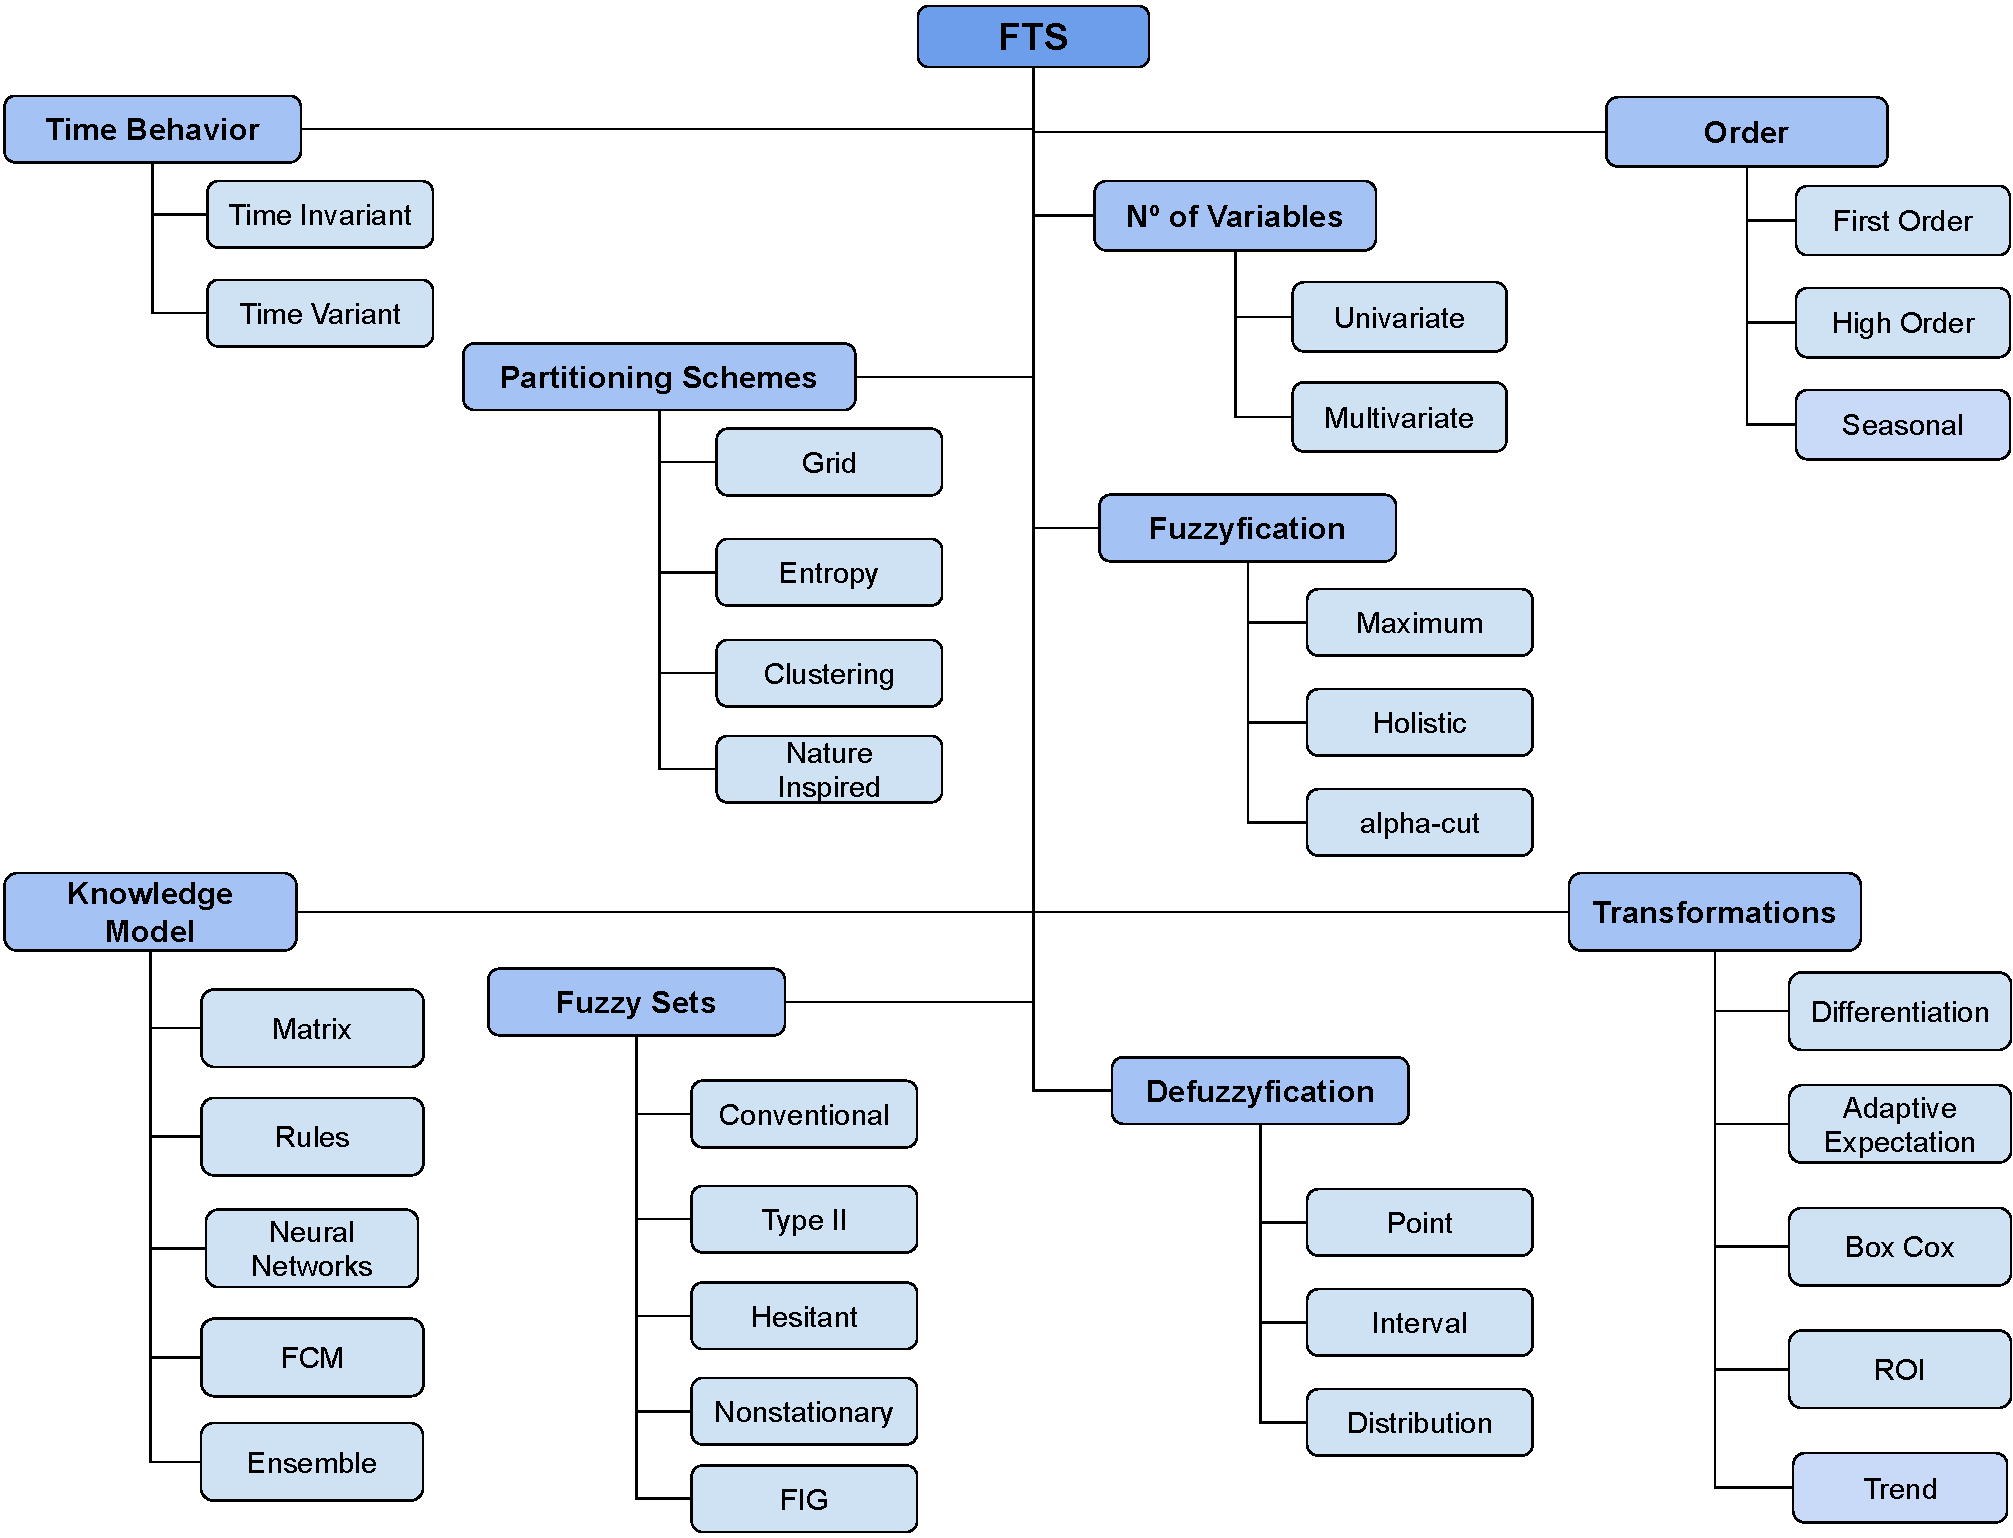
\includegraphics[width=\textwidth, height=15cm]{figures/fts_taxonomy.pdf}
    \caption{A brief taxonomy of FTS methods}
    \label{fig:fts_taxonomy}
\end{figure}

The most important categories of FTS methods are related with their the time behavior. The time invariant models are the ones used when the Universe of Discourse and data behavior  does not change with time, as in stationary time series. Non stationary time series, in its turn, require time variant models as proposed in \cite{Song1994} and \cite{Wong2010}. This research is focused on time invariant models and hereinafter all models discussed belongs to it. However, Time Variant models are not discarded for future investigations.

The main contributions of this chapter are the proposals of two consensus methods, which aggregate the major developments of the FTS literature for high order rule based and weighted rule based methods: the High Order Fuzzy Time Series (HOFTS) and the Weighted High Order Fuzzy Time Series (WHOFTS). These methods are intended for point forecasting, for one to many steps ahead.

This chapter also focus only on monovariate and non Big Data time series. The multivariate and Big Data methods will be discussed in the following chapters. In the next section the main processes of the FTS are introduced and discussed.

%%%%%%%%%%%%%%%%%%%%%%%%%%%%%%%%%%%%%%%%%%%%%%%%%%%%%%%%%%%%%%%%%%%%%%%%%%%%
%%%%%%%%%%%%%%%%%%%%%%%%%%%%%%%%%%%%%%%%%%%%%%%%%%%%%%%%%%%%%%%%%%%%%%%%%%%%

\section{Fuzzy Time Series common processes}
\label{sec:common_fts} \index{Common Fuzzy Time Series processes}\index{FTS process}

\index{Universe of Discourse}\index{UoD}\index{Fuzzy Time Series}\index{FTS}

The definition of Fuzzy Time Series, from \cite{song1993fuzzy}, starts with a univariate time series $Y \in \mathbb{R}^1$, for $t = 0,1,...,T$, where the Universe of Discourse $U$ is delimited by the known bounds of $Y$, such that $U = [\min(Y),\max(Y)]$. Upon $U$, $k$ fuzzy sets $\ufset$, for $j = 1..k$, are defined and each one with its own membership function $\mu_{\ufset}$. $F$ is called a Fuzzy Time Series over $Y$ if $f(t) = \mu_{\ufset}(y(t))$ is the collection of fuzzyfied values of $Y$ for $j = 1..k$ and $t = 0,1,...,T$. The group of fuzzy sets $\ufset$, for $j = 1..k$, can also be understood as a Linguistic Variable $\ulvar$, and each fuzzy set $\ufset \in \ulvar$ is a linguistic value of the linguistic variable. 
\index{Linguistic Variable}

\begin{figure}[htb]
    \centering
    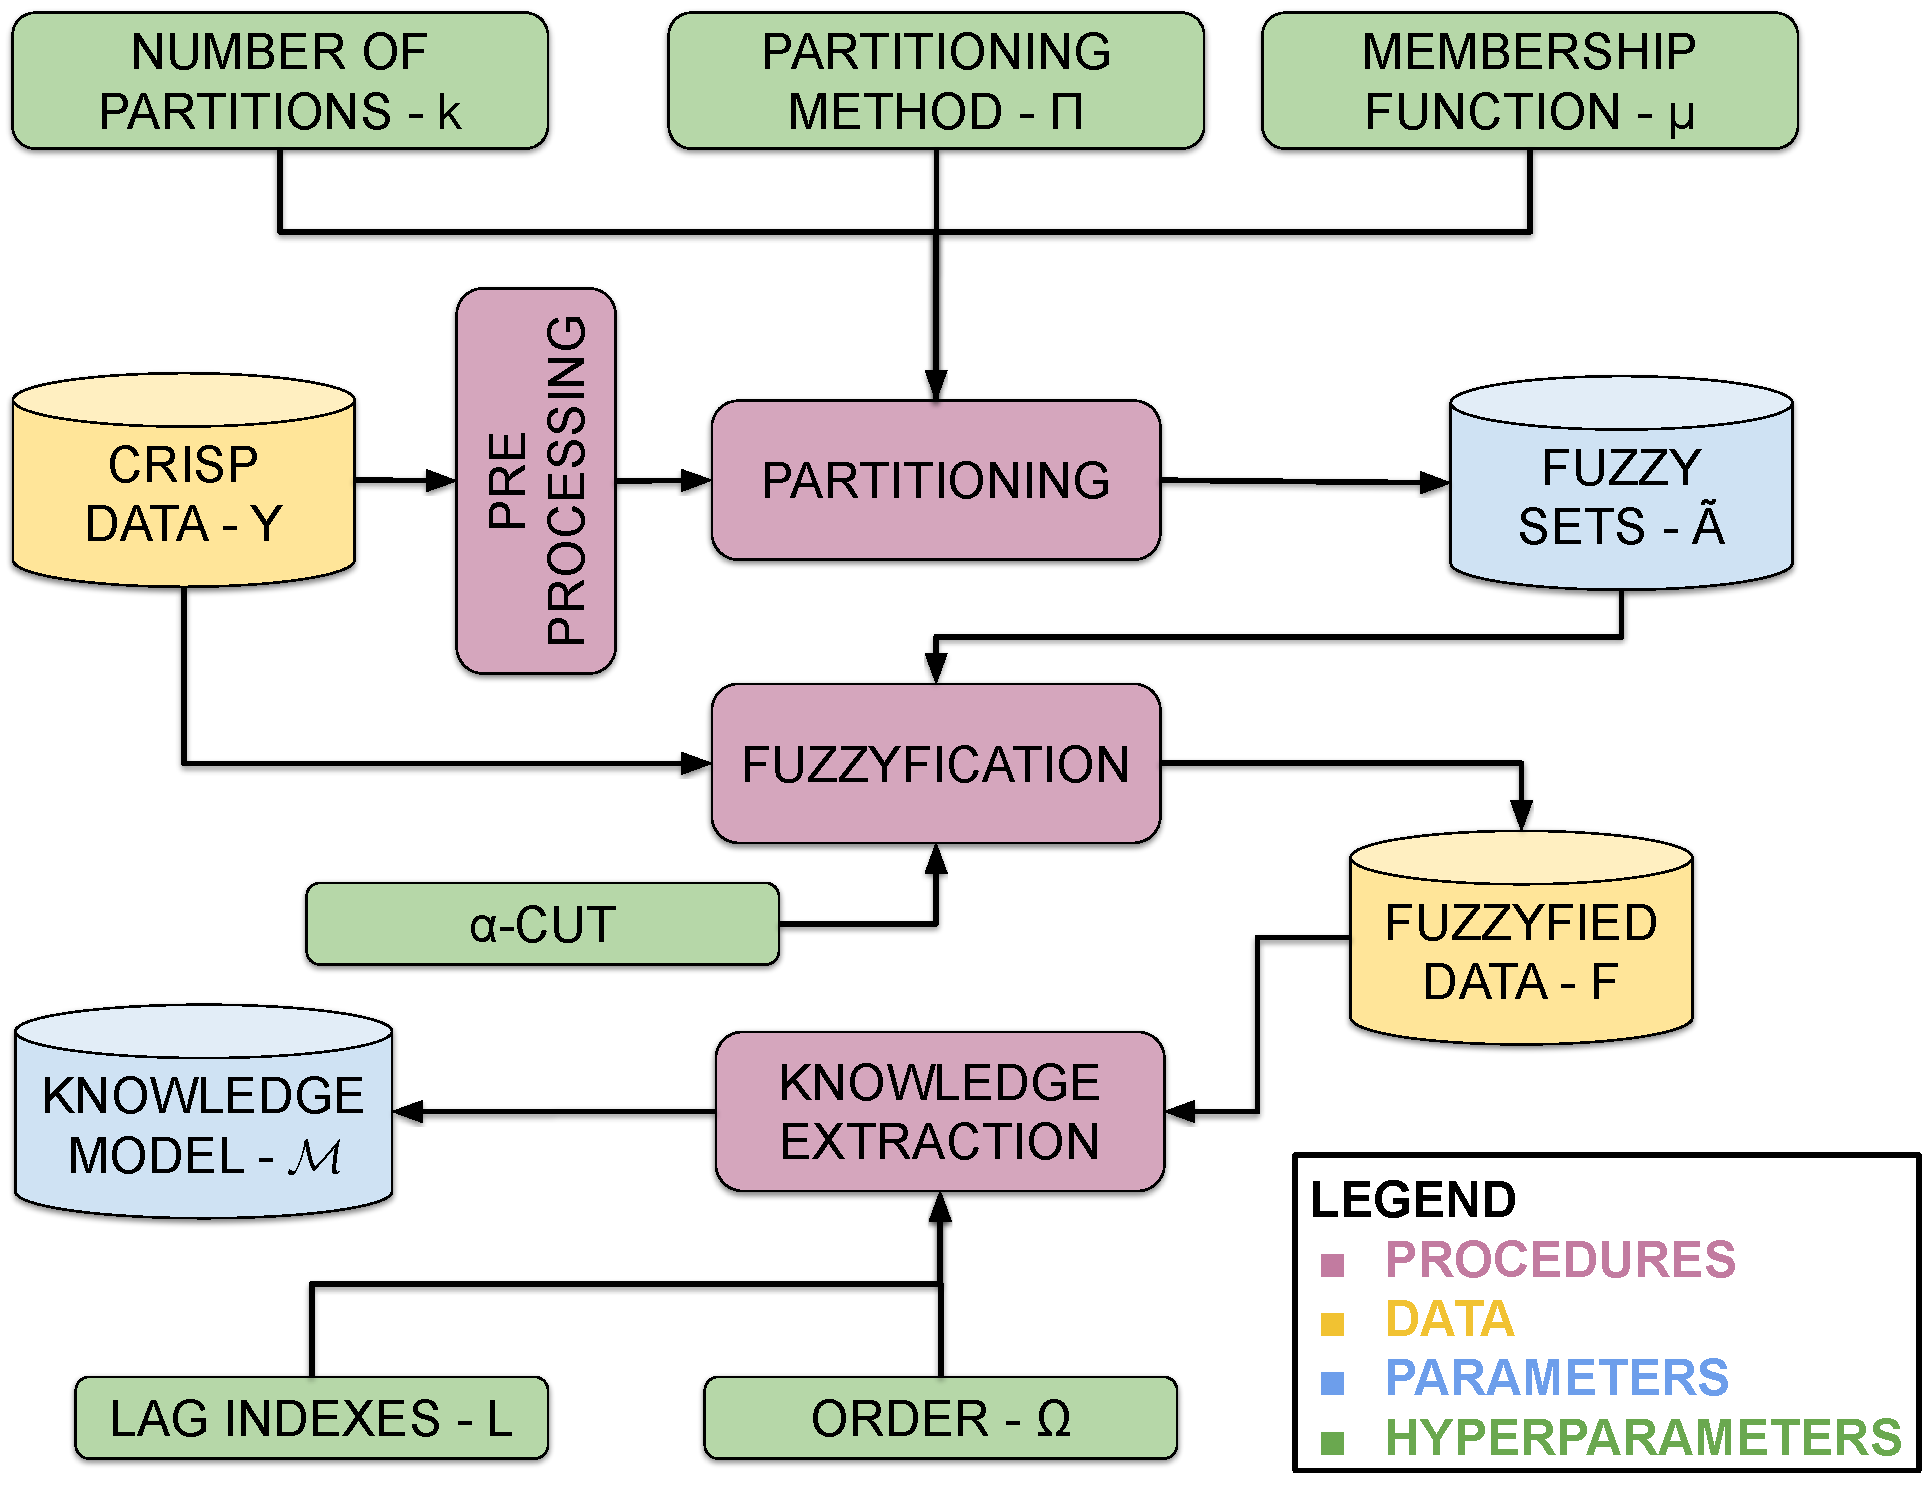
\includegraphics[width=\textwidth]{figures/fts_training.pdf}
    \caption{Generic time invariant Fuzzy Time Series training procedure and its components}
    \label{fig:fts_training}
\end{figure}

\cite{Song1993partI} proposed the first FTS methodology and the following authors basically extended or modified some steps of the method. A generic method can be extracted from the wide range of variations of FTS methods by splitting the FTS approach in two main procedures, the training and forecasting methods. The training method, illustrated in Figure \ref{fig:fts_training}, has the basic objective to create the linguistic variable $\ulvar$ and a knowledge representation of the time series dynamics. These two objects compose the FTS model $\model$. The main components of this process are listed below:

\begin{enumerate}
    \item[Step 1] - \textbf{Pre-processing}: First, one or more pre-processing data transformations can be applied to input data $Y$, responsible to reduce noise, detrending, or de-seasonalize, or change the $U$, etc. Several methods contain these operators and their impact will be discussed in detail in Section \ref{sec:fts_transformations}.
    
    \item[Step 2] - \textbf{Partitioning}: The most important process of the training is executed, the partitioning. This process is responsible to split the universe of discourse $U$ into $k$ fuzzy sets $\ufset$, creating the linguistic variable $\ulvar$ used to describe $Y$. There are many ways that the partitioning can be performed, and the most important are discussed in Section \ref{sec:fts_partitioning}.
    
    \item[Step 3] - \textbf{Fuzzyfication}: With the linguistic variable $\ulvar$ the crisp data $Y$ can be transformed in a linguistic representation, the fuzzy time series $F$ where each $f(t) \in F$ is a fuzzyfied version of $y(t) \in Y$. Details of the fuzzyfication are discussed in Section \ref{sec:fts_fuzzyfication}.
    
    \item[Step 4] - \textbf{Knowledge Extraction and Representation}: The second most important process is the knowledge extraction. This process is responsible to induce the knowledge model $\model$ by performing a pattern recognition over $F$ and learning the temporal patterns between  $\Omega$ lags, whose indexes are identified by $L$, and their consequent ones. The most important learning algorithms and knowledge models are discussed in Section \ref{sec:fts_knowledge}.
\end{enumerate}

Once the linguistic variable $\ulvar$ is defined and the FTS model $\model$ was learned, new samples $y(t) \in U$ can be presented to produce a forecast $\hat{y}(t+1)$. The generic forecasting procedure is illustrated in Figure \ref{fig:fts_forecasting}, and its main components are listed below:

\begin{enumerate}
    \item [Step 1] - \textbf{Pre-processing}: First, one or more pre-processing and post-processing data transformations can be applied to input sample $y(t)$ (the data transformations are discussed in Section \ref{sec:fts_transformations}).
    
    \item[Step 2] - \textbf{Fuzzyfication}: The fuzzyfication procedure follows the same schema of the training procedure and it is discussed in Section \ref{sec:fts_fuzzyfication}. 
    
    \item[Step 3] - \textbf{Inference}: The inference engine deeply depends on the knowledge model $\model$. Indeed, the learning algorithm, the knowledge model and the inference engine are intrinsically correlated, and they are discussed in Section \ref{sec:fts_knowledge}. The aim of the inference process is to produce $f(t+1)$, candidate fuzzy sets (and other additional information, as weights) to represent the future crisp value $y(t+1)$.
    
    \item[Step 4] - \textbf{Deffuzyfication}: The deffuzyfication process aims to transform the $f(t+1)$ to a crisp numeric estimate $\estimate$ for the real (but unknown) value $y(t+1)$. The deffuzyfication usually also depends on the inference engine but there are common methods discussed in Section \ref{sec:fts_defuzzyfication}. The present work extended the possibilities of deffuzyfication to beyond of point forecasting, proposing methods for prediction intervals $\mathbb{I}$ and probabilistic distributions $P$.
    
    \item [Step 5] - \textbf{Post-processing}: Finally, one or more post-processing data transformations can be applied to output forecast $\estimate$  (the data transformations are discussed in Section \ref{sec:fts_transformations}).
\end{enumerate}

\begin{figure}
    \centering
    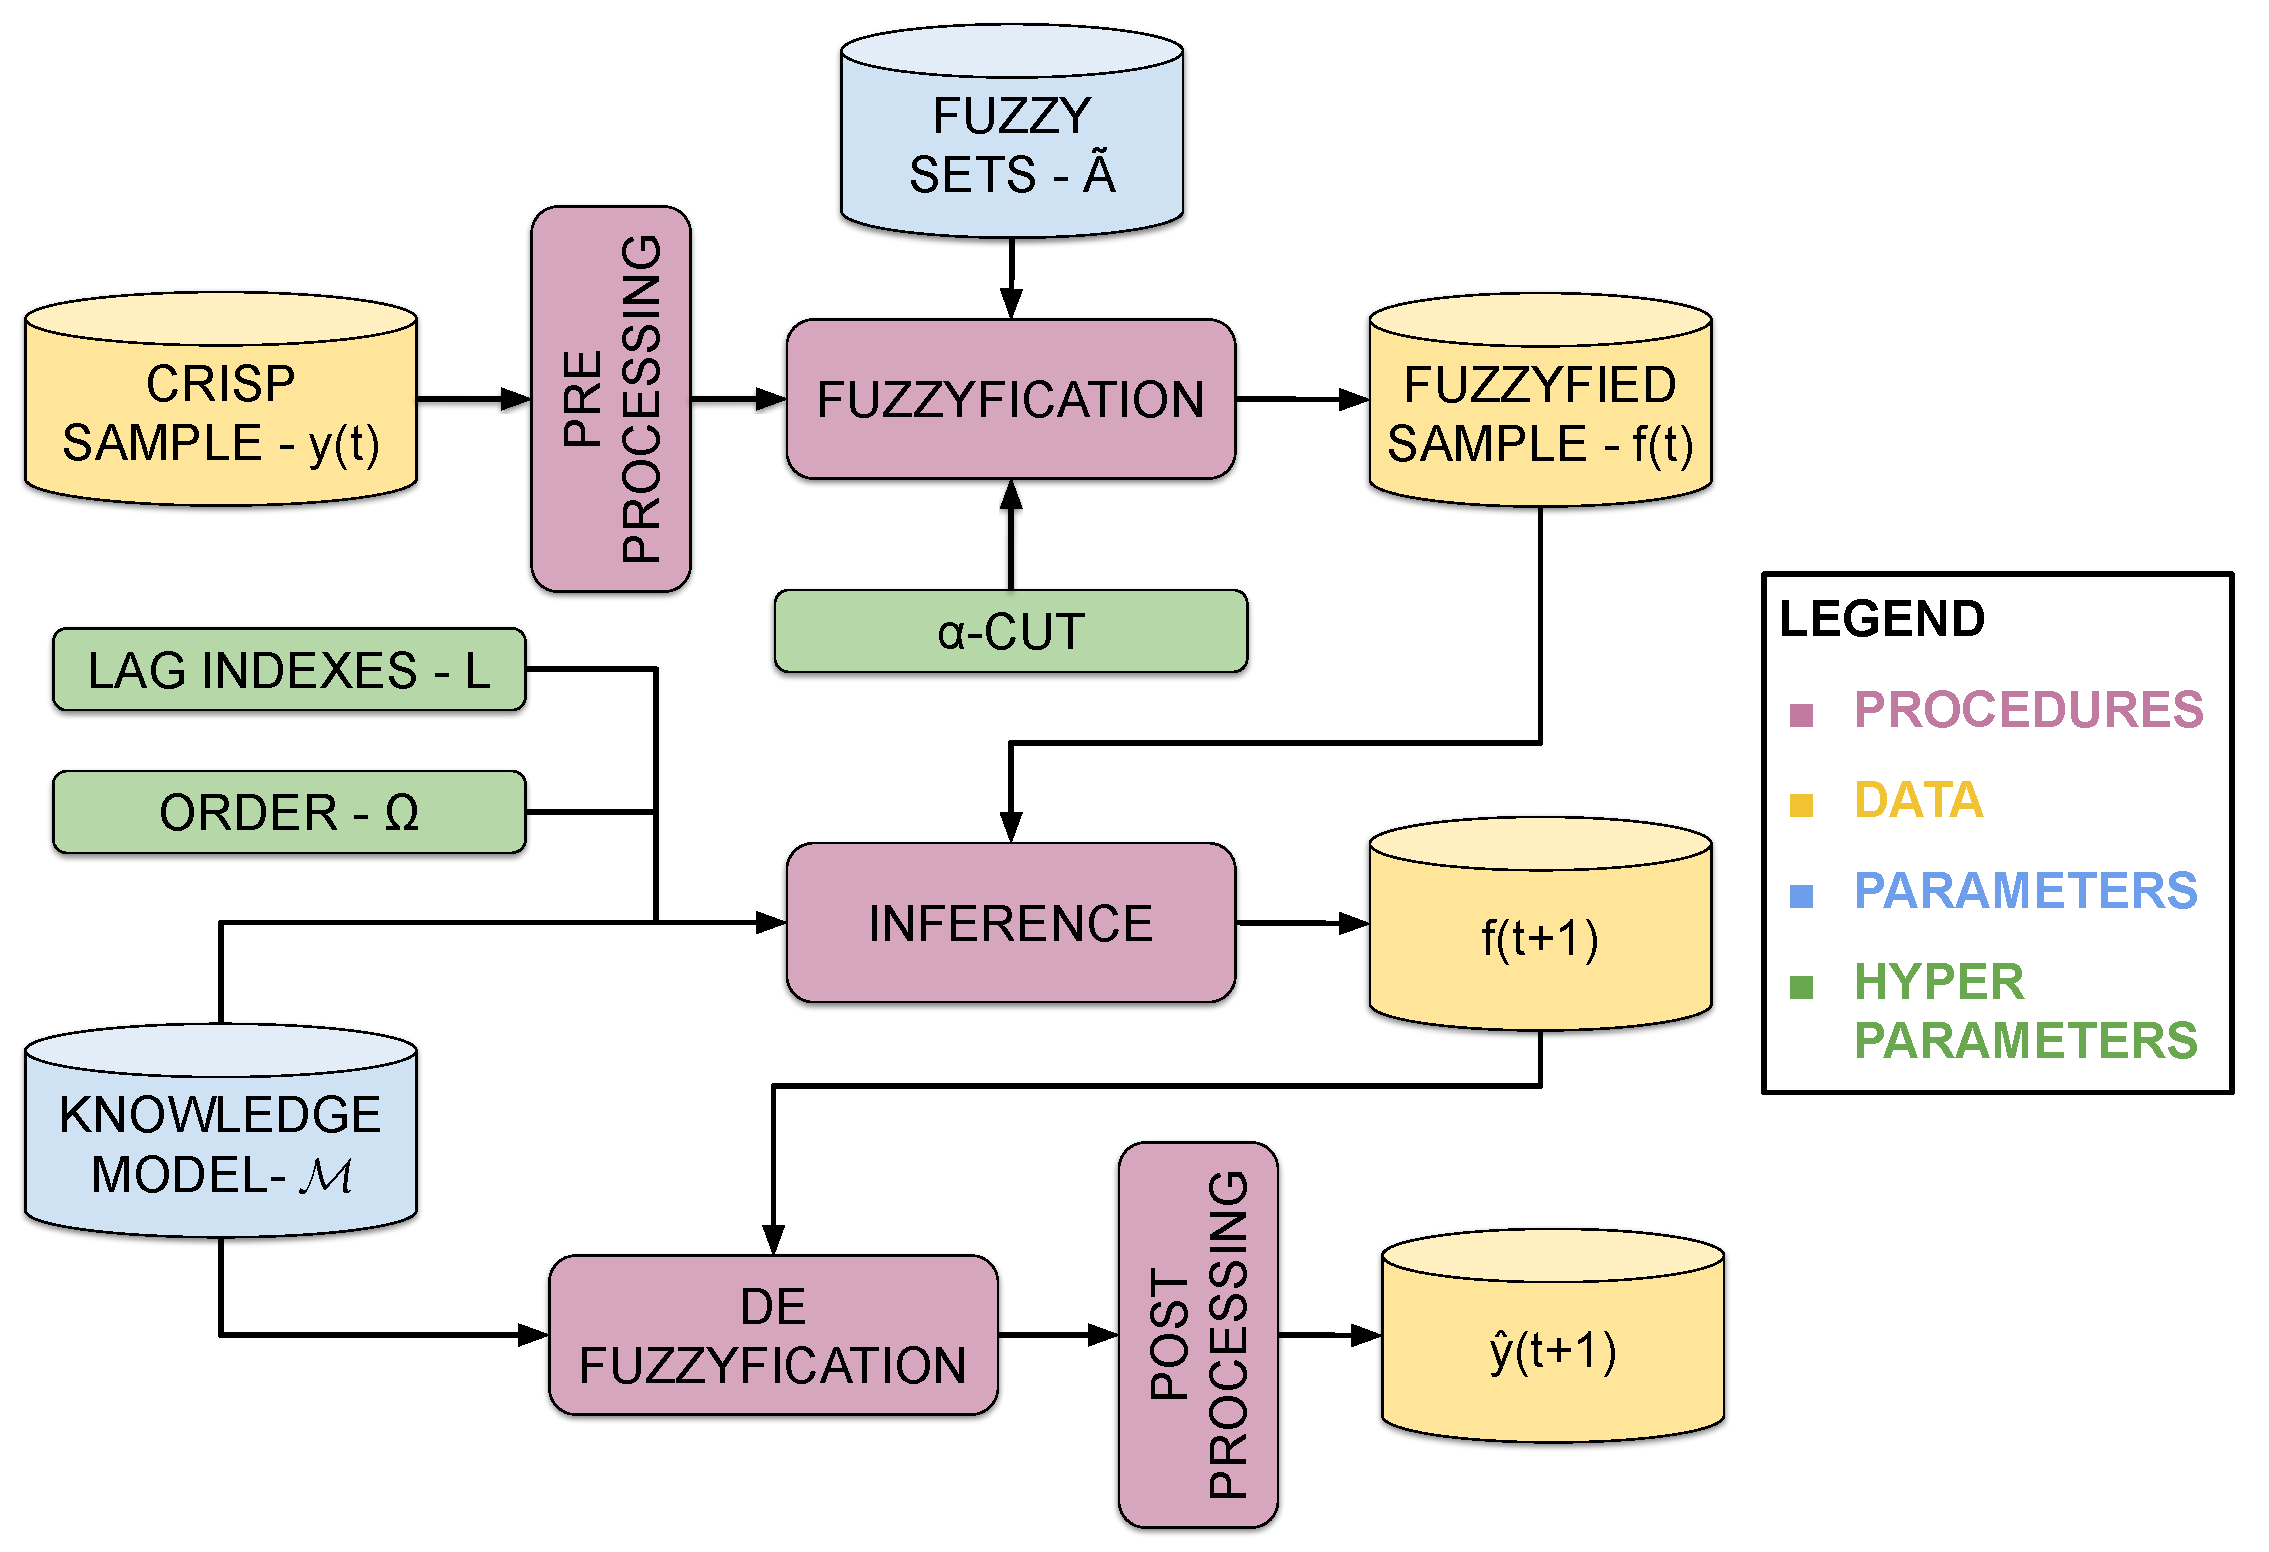
\includegraphics[width=\textwidth,height=12cm]{figures/fts_forecasting.pdf}
    \caption{Generic time invariant Fuzzy Time Series forecasting procedure and its components}
    \label{fig:fts_forecasting}
\end{figure}


The main hyperparameters which affect these processes are listed in Table \ref{tab:fts_hyperparameters}. The selection of the values for these hyperparameters affects the training process and the parameters of the model, including its accuracy and parsimony (the length of the model).  In the following sections each one of these processes are discussed in detail recurring to the most relevant works in the FTS literature, while its strengths and drawbacks are highlighted.

\begin{table}[]
    \centering
    \begin{tabular}{|c|m{7cm}|m{5cm}|} \hline
        \textbf{Alias} & \textbf{Parameter}& \textbf{Process} \\ \hline
         $k \in \mathbb{N}^+$ & Number of partitions (fuzzy sets) & Universe of Discourse Partitioning \\ \hline
         $\mu: U \rightarrow [0,1] $ & Membership function, measures the membership of a value $y \in U$ to a fuzzy set & Universe of Discourse Partitioning, Fuzzyfication  \\\hline
         $\Pi$ & Partitioning method & Universe of Discourse Partitioning \\\hline
         $\alpha \in [0,1]$ & the $\alpha$-cut, the minimal membership grade to take account on fuzzyfication process & Fuzzyfication \\ \hline
         $\Omega \in \mathbb{N}^+$ & Order, the number of lags & Knowledge model  \\\hline
         $L \in \Omega \times \mathbb{N}^-$ & Time lag indexes & Knowledge model \\\hline
    \end{tabular}
    \caption{Common hyperparameters for FTS methods}
    \label{tab:fts_hyperparameters}
\end{table}

\index{Hyperparameter}

%%%%%%%%%%%%%%%%%%%%%%%%%%%%%%%%%%%%%%%%%%%%%%%%%%%%%%%%%%%%%
%
%%%%%%%%%%%%%%%%%%%%%%%%%%%%%%%%%%%%%%%%%%%%%%%%%%%%%%%%%%%%%
\section{Universe of Discourse Partitioning}
\label{sec:fts_partitioning}
\index{UoD Partitioning}\index{Partitioning Schemes}

This process aims to split the Universe of Discourse $U$ and to create the linguistic variable $\ulvar$, composed by the fuzzy sets $\ufset$, $j = 1 .. k$. This is the most important process of the FTS approach and the following sections detail its main sub-processes and parameters.

%%%%%%%%%%%%%%%%%%%%%%%%%%%%%%%%%%%%%%%%%%%%%%%%%%%%%%%%%%%%%
%
%%%%%%%%%%%%%%%%%%%%%%%%%%%%%%%%%%%%%%%%%%%%%%%%%%%%%%%%%%%%%
\subsection{Universe of Discourse $U$}
\label{sec:fts_uod} \index{Universe of Discourse}\index{$U$}\index{UoD}

The natural definition of the Universe of Discourse is $U = [\min(Y),\max(Y)]$, but it is common that the upper and lower bounds be exceeded by a confidence margin. Then, it can be established as $U = [\underline{l}, \overline{u}]$, with the lower bound as $\underline{l} = \min(Y) + l_d$, where $l_d = \min(Y)\cdot 0.2$ (exceeding the original lower bound by 20\%) and the upper bound as $\overline{u} = \max(Y) + u_d$, where $u_d = \max(Y)\cdot 0.2$ (exceeding the original upper bound by 20\%). 

Even considering just time invariant methods in this work and a stationary time series $Y$, it is natural that the testing $U$ will be a little different from the training $U$, sometimes by a small fraction of the original values. Even on stationary processes the presence of outliers cannot be discarded. The objective of these exceeding margins $l_d$ and $u_d$ is to help in the fuzzyfication process of the forecasting procedure, in order to accommodate fluctuations in the bounds of the known $U$.

%%%%%%%%%%%%%%%%%%%%%%%%%%%%%%%%%%%%%%%%%%%%%%%%%%%%%%%%%%%%%
%
%%%%%%%%%%%%%%%%%%%%%%%%%%%%%%%%%%%%%%%%%%%%%%%%%%%%%%%%%%%%%
\subsection{Membership function $\mu$}\index{Membership function}\index{$\mu$}\index{Fuzzy sets}
\label{sec:fts_membership}

Once $U$ has been defined, three hyperparameters will determine the creation of $\ulvar$: the number of partitions $k$, the membership function $\mu$ and the partitioning scheme. The membership function $\mu: U \rightarrow [0,1]$ defines how much a crisp value belongs to a fuzzy set, in terms of the membership grade $[0,1]$. Some options of fuzzy membership functions are shown in Table \ref{tab:fts_membership}, and simple partitioning using these functions are shown in Figure \ref{fig:membership}. The real impact of the membership function on accuracy is low, it will be demonstrated empirically later on this work, but the chosen of the correct $\mu$ can help in the readability and explainability of the model.

Many other kinds of fuzzy sets were presented in the literature and new FTS methods were developed using them, as instance Type 2 fuzzy sets \citep{huarng2005type, Bajestani2011}, Hesitant fuzzy sets \citep{Bisht2016}, non-stationary fuzzy sets \citep{Alves2018}, etc. These fuzzy sets and the methods developed with them, however, are considered out of the scope of this research.

\index{Membership function}\index{$\mu$}
\begin{table}[]
    \centering
\begin{tabular}{|c|m{4cm}|c|} \hline
\textbf{Name}  & \textbf{Parameters}  & \textbf{Definition} \\ \hline
Singleton  & $c$, the central value & 
$\mu(x,c) = \left\{ \begin{array}{ccc}
        1 & if & x = c  \\
        0 & if & x \neq c
    \end{array}\right.$ \\ \hline
Triangular  & $a$: lower bound, $b$: midpoint, $c$: upper bound  & 
$\mu(x,a,b,c) = \left\{ \begin{array}{ccc}
        0 & if & x \leq a  \\
        \frac{x-a}{b-a} & if & a \leq x \leq b  \\
        \frac{c-x}{c-b} & if & b \leq x \leq c  \\
        0 & if & c \geq x
    \end{array}\right.$ \\ \hline
Trapezoidal  & $a$: lower bound, $b$: top-left, $c$: top-right, $d$ upper bound & 
$\mu(x,a,b,c,d) = \left\{ \begin{array}{ccc}
        0 & if & x \leq a  \\
        \frac{x-a}{b-a} & if & a \leq x \leq b  \\
        1 & if & b \leq x \leq c  \\
        \frac{d-x}{d-c} & if & c \leq x \leq d  \\
        0 & if & d \geq x
    \end{array}\right.$ \\ \hline
Gaussian  & $m$: midpoint, $d$: spread & 
$\mu(x,m,d) = \exp \left(-\frac{(x-d)^2}{2m^2}\right)$ \\ \hline
\end{tabular}
\caption{Most common fuzzy membership functions}
    \label{tab:fts_membership}
\end{table}

\begin{figure}
    \centering
    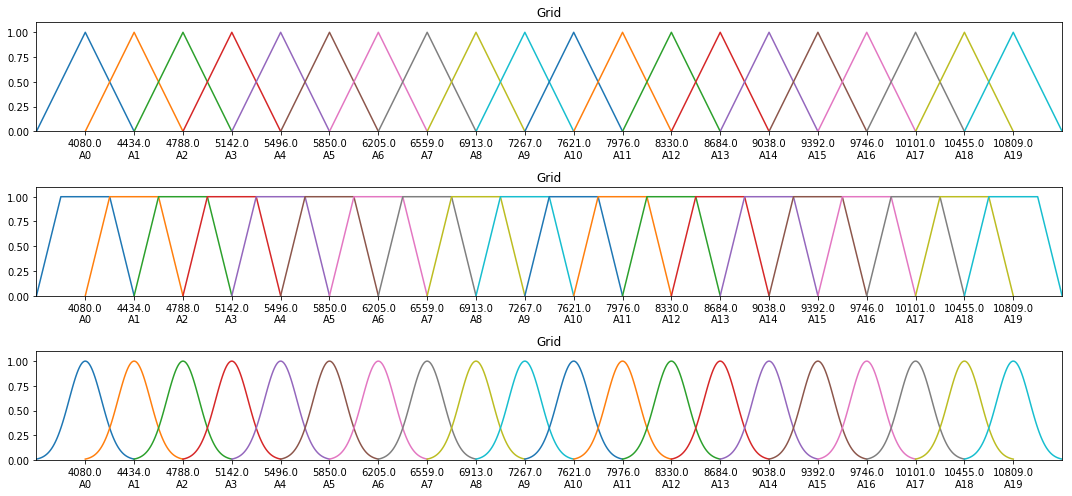
\includegraphics[width=\textwidth]{figures/membership.png}
    \caption{UoD Partitioning using different membership functions}
    \label{fig:membership}
\end{figure}

%%%%%%%%%%%%%%%%%%%%%%%%%%%%%%%%%%%%%%%%%%%%%%%%%%%%%%%%%%%%%
%
%%%%%%%%%%%%%%%%%%%%%%%%%%%%%%%%%%%%%%%%%%%%%%%%%%%%%%%%%%%%%
\subsection{The number of partitions $k$}\index{Number of partitions}\index{$k$}
\label{sec:fts_partitions}

\index{overfit}\index{underfit}\index{Hyperparameter Optimization}\index{model accuracy}\index{model performance}
The selection of the hyperparameter $k$ impact directly on the model accuracy and parsimony, as discussed in \cite{Duru2012}. The number of partitions impact on the model parsimony directly and, for instance, given a rule model the maximum number of rules is the cartesian product between the fuzzy sets $\ufset \in \ulvar$ for each order $\Omega$. 

There is a non-linear relationship between $k$ and the model accuracy, a trade off between specific accuracy (bias) and overall generalization (variance). A small value of $k$ will generate too few fuzzy sets to represent $Y$ correctly, making the model $\model$ underfit by producing a gross generalization with simplistic patterns. A high value of $k$ will generate too much fuzzy sets, exceeding the needed to represent $Y$ and makeing the model $\model$ overfit by reproducing excessive specificities and small noisy fluctuations. The optimal number of $k$ must be optimized for each problem, balancing the accuracy and the model parsimony, since this last value affects the computational performance as the number of parameters grows.

The impact of the $U$ partitioning can also be seen by other perspectives: the model human readability and model explainability. In his seminal work, \cite{Miller1956} stated that the human being, on average, can learn $7 \pm 2$ concepts. In other words, the linguistic variable $\ulvar$ to be reasonable for human understanding must have around this number of fuzzy sets. But this, depending on the range of $U$ and the behavior of $Y$, may be a very small number of partitions. Otherwise, the explainability does not depend on how much humans can learn from $\model$ but how easily the forecastings produced can be explained, as a white box model. In this last case the type of the knowledge representation of $\model$ has greater impact than the number of fuzzy sets in $\ulvar$. 

A study of the linguistic characterization of time series can be found in \cite{Novak2016}. using Fuzzy Transform (\cite{Perfilieva2006}) to generate linguistic summaries of time series. A study on mining information from fuzzyfied linguistic time series can be found in \cite{Novak2016a}, where are presented the impacts of fuzzyfication on the knowledge extraction.

%%%%%%%%%%%%%%%%%%%%%%%%%%%%%%%%%%%%%%%%%%%%%%%%%%%%%%%%%%%%%
%
%%%%%%%%%%%%%%%%%%%%%%%%%%%%%%%%%%%%%%%%%%%%%%%%%%%%%%%%%%%%%
\subsection{The partitioning method - $\Pi$}\index{UoD Partitioning}\index{Partitioning Method}\index{$\Pi$}\index{Fuzzy sets}
\label{sec:fts_partitioningmethod}

The partitioning method will determine, for each fuzzy set,  their length, midpoints and bounds and also have impact on accuracy. The simplest partitioning scheme -- the division of the data range in $k$ equal length intervals -- is called Grid Partitioning and was proposed in \cite{song1993fuzzy}. \index{Grid Partitioning} In the Grid Partitioning, $U$ is divided in $k+2$ even intervals $u_1, u_2, ..., u_k$ whose midpoints are $c_1, c_2, ..., c_k$. Then with these $k$ intervals $k$ overlapped fuzzy sets $A_1,A_2,...,A_k$ are defined using triangular membership functions whose parameters are $c_{j-1},c_j,c_{j+1}$ for each $j = 2..k-1$. 

Some works used simple heuristics to define $k$ or even the lengths of the fuzzy sets. \cite{huarng2001effective}\index{Huarng Partitioning}\index{Heuristic Partitioning} use a grid partitioning approach, but it proposes an empirical method to find the ideal number of partition lengths according to the magnitude of $U$, in a work that was the first to deeply discuss the impact of the partitioning on FTS forecast accuracy. Several other works used this or define other simple heuristic for $U$ partitioning, see for instance \cite{Chang1997, huarng2005type, Rubio2016, Cheng2018}.

$U$ partitionings where the fuzzy sets have unequal lengths are also present in the literature. \cite{Cheng2006a} employ a fixed value of $k$ but the entropy of data that defines the best midpoints for the fuzzy sets, which also use trapezoidal membership functions. This method is known by Entropy Partitioning and is also employed in \cite{Cheng2008} and \cite{Chen2014}.\index{Entropy Partitioning} The statistical approaches yet count with \cite{Ismail2015}, which determine the length of the fuzzy sets proposing a method based on data quantiles, and \cite{Yang2017} which use a Chi-Square distribution do identify the fuzzy sets number and lengths.

Clustering techniques are used in several works, as Fuzzy C-Means in \cite{Li2008b, Askari2015, Bas2015, Sun2015, Yolcu2017}, Fuzzy K-Medoids in \cite{Dincer2018}, Self Organizing Maps in \cite{Bahrepour2011}, and other methods as in \cite{Saberi2017} and \cite{Bose2017}.\index{FCM Partitioning}\index{Cluster Partitioning}

The use of metaheuristics, especially of nature-inspired optimization approaches, is also spread in the literature. Particle Swarm Optimization is used by \cite{Davari2009, Kuo2009, Hsu2010, Huang2011, Zhang2018a}, Genetic Algorithms in \cite{Chen2006a, Enayatifar2013, Zhang2018}, and other less known methods such as Harmony Search in \cite{Talarposhti2016a, Jiang2017} and Imperialist Competitive in \cite{Sadaei2017}. \index{Evolutionary Partitioning}\index{Metaheuristic Partitioning}\index{PSO Partitioning}

\begin{figure}
    \centering
    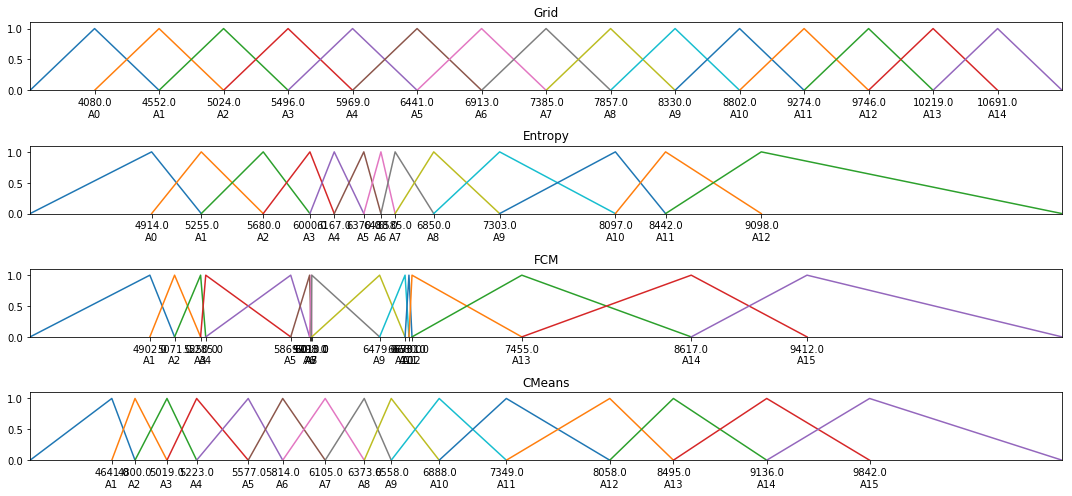
\includegraphics[width=\textwidth]{figures/partitioners.png}
    \caption{Partitioning using different approaches within the same sample}
    \label{fig:partitioners}
\end{figure}

A sample of different partitioning schemes on the same data can be seen in Figure \ref{fig:partitioners}. The partitioning method has influence on the model accuracy, parsimony and readability but its computational cost must be also considered. The Grid Partitioning gives a uniform distribution of the fuzzy sets over $U$ but, if in one hand it is computationally cheaper, however it may not represent the importance of some data regions accordingly. It is probable that some specific regions of $U$ have more variance than others, depending on $Y$ behavior, and some regions may be better represented having more fuzzy sets than others. It also can not be denied that some approaches are computationally expensive, as the clustering and metaheuristics ones, and in Big Data scenarios this may be prohibitive. Despite the fact that the Grid Partitioning should be always the first approach to start with, due to its simplicity and small cost, the fine tuning of FTS models can not exclude more sophisticated methods.

Once the linguistic variable $\ulvar$ is created, the fuzzyfication process can be started. This process and its parameters are discussed in the next section.


%%%%%%%%%%%%%%%%%%%%%%%%%%%%%%%%%%%%%%%%%%%%%%%%%%%%%%%%%%%%%
%
%%%%%%%%%%%%%%%%%%%%%%%%%%%%%%%%%%%%%%%%%%%%%%%%%%%%%%%%%%%%%
\section{The Fuzzyfication Process}
\label{sec:fts_fuzzyfication}
\index{Fuzzyfication Method}\index{Fuzzy sets}

This process aims to transform the crisp numerical time series $Y$ into a linguistic time series $F$, also known as fuzzy time series. There are few, but important, variations of the fuzzyfication method.

The initial FTS methods, for instance \cite{song1993fuzzy}, \cite{chen1996forecasting} and \cite{yu2005weighted}, only considered one fuzzy set in fuzzyfication process, for instance $y(t) \in Y$, the one with the greatest membership grade. More specifically:
\index{Maximum membership fuzzyfication}

\begin{equation}
f(t) = \ufset\; |\; \mu_{\ufset}(y(t)) = \max\{ \mu_{A_1}(y(t)), \ldots, \mu_{A_k}(y(t)) \}    
\label{eqn:fuzzyfication_maximum}
\end{equation}

\index{overfit}\index{underfit}
This method helps to control overfit, reducing the number of spurious patterns generated by low membership grades fuzzy sets. However, it can also contribute to underfit the learning by eliminating fuzzy sets which are very close to the maximum grade. It is possible to deduce that some relevant information can be lost when several minor membership grades are discarded.

A contrasting method is the holistic fuzzyfication, where all the membership grades, despite their magnitude, are considered. The fuzzyfied value $f(t)$ is the the vector of the $y(t)$ membership grades with respect to each $\ufset \in \ulvar$:

\begin{equation}
f(t) = [\mu_{A_1}(y(t)), \ldots, \mu_{A_k}(y(t)) ]    
\label{eqn:fuzzyfication_holistic}
\end{equation}

\index{Alpha cut}\index{$\alpha$-cut}\index{Holistic fuzzyfication}
The holistic fuzzyfication can help to the learning overfit, because even very small membership grades, which can be considered insignificant for that fuzzy set, are considered. An intermediate approach can be achieved by using the $\alpha$-cut hyper-parameter. The $\alpha$-cut represents the minimal value of the membership grade that will be accepted in fuzzyfication, while membership values below the $\alpha$-cut will not be considered. 

\begin{equation}
f(t) = \ufset\; |\; \mu_{\ufset}(y(t)) \geq \alpha \;\; \forall \ufset \in \ulvar    
\label{eqn:fuzzyfication_alpha}
\end{equation}

The $\alpha$-cut makes the sensibility of the fuzzyfication process adjustable and the user can control it, unlike the maximum membership and the holistic methods. The fuzzyfication method is significant in the search of the training best fit, controlling the accuracy and models parsimony. Particularly, the method of \cite{CarvalhoJr2017} makes an explicit use of the $\alpha$-cut parameter and conduct a comprehensive study of its impact on the method accuracy.

Once the crisp data $Y$ is converted to the fuzzy time series $F$ the process of knowledge extraction and representation is ready to start. This process and its variations are discussed in the next section.

%%%%%%%%%%%%%%%%%%%%%%%%%%%%%%%%%%%%%%%%%%%%%%%%%%%%%%%%%%%%%
%
%%%%%%%%%%%%%%%%%%%%%%%%%%%%%%%%%%%%%%%%%%%%%%%%%%%%%%%%%%%%%
\section{Knowledge Extraction, Representation and Inference}
\label{sec:fts_knowledge}
\index{Knowledge extraction}\index{Knowledge representation}
\index{Inference}\index{Induction}

This section aims to investigate the several approaches in the literature that were used to learn and represent temporal patterns found on the fuzzyfied data $F$. Looking back to Figures \ref{fig:fts_training} and \ref{fig:fts_forecasting}, the fuzzy sets and the fuzzyfication process may be interpreted as a feature extraction layer that precedes a pattern recognition and inference layer, that is finally succeeded by a reconstruction layer -- the deffuzyfication process. Besides small variations, the fuzzyfication and deffuzyfication do not differ among the methods. But the way these methods learn and store the patterns suffer a strong variation among them.

By far, most of FTS methods make use of simple heuristics to learn the temporal patterns from the fuzzyfied data and store the learned patterns using rules or matrices. But it can not be denied that there are many other backends for the knowledge extraction and representation in FTS models: metaheuristics, neural networks, fuzzy cognitive models, hybrid approaches with traditional statistical models, etc. In the following sections the most relevant methods with their variations will be discussed. 

%%%%%%%%%%%%%%%%%%%%%%%%%%%%%%%%%%%%%%%%%%%%%%%%%%%%%%%%%%%%%
%
%%%%%%%%%%%%%%%%%%%%%%%%%%%%%%%%%%%%%%%%%%%%%%%%%%%%%%%%%%%%%
\subsection{The Order $\Omega$, Lags $L$ and Seasonality}
\label{sec:fts_order}\index{High Order Models}\index{Lags}\index{Seasonal Models}\index{$\Omega$}\index{$L$}

First it is needed to consider the hyperparameters order $\Omega$ and the lag indexes $L$. These parameters also impact directly on the model accuracy and parsimony. The number of lags $\Omega$ indicate how much past information is available to the model $\model$ to recognize the possible temporal patterns and make a forecast. Very short-term memory or even memory-less processes will require just the last time lag, consequently produce a first order model ($\Omega = 1$). Processes with longer memories will require more lags and produce higher-order models ($\Omega>1$). 

Otherwise, the hyperparameter $L$ indicates which past lags are taken into account during the forecast. Not always the most recent time lags contain the best information to predict the near future and this is particularly important for seasonal time series, where $L$ will indicate the time lags which have periodically similar values. Initially the values of $L$ can be extracted from the Autocorrelation Function (ACF), examining the most significant lags. However, this number can be optimized with fewer lags.

\index{Seasonal Fuzzy Time Series}\index{SFTS}\index{High Order Fuzzy Time Series}\index{HOFTS}

The \textit{High Order Fuzzy Time Series} - HOFTS  defines the High Order Fuzzy Logical Relationships - HOFLR as $LHS \rightarrow RHS$ form, where $LHS$ is the set of $f(t-L(\Omega-1)), ..., F(t - L(0))$ fuzzy sets, and the $RHS$ is $f(t+1)$, the group of consequent fuzzy sets. We can find these kind of models in \cite{Chen2002, Chen2006a, Jilani2008a, Li2008b, Egrioglu2010, Bahrepour2011, Enayatifar2013, Chen2014, Chen2015a, Ye2016, Lee2017, Bose2017, Sadaei2017, Guney2018, Cheng2018, Yang2018, Zhang2018a}.


Seasonal models try to represent cyclical behaviors, e. g, repeated values of the time series in regular periods. \textit{Seasonal Fuzzy Time Series} - SFTS methods, make use of the $L$ parameter to represent the seasonal periods as lag indexes. SFTS were first proposed  in \cite{Song1997}, basically by defining a seasonal index in $L$, such that $f(t+1) = f(t-L)$. \cite{Chang1997} proposed a method for capturing fuzzy trend and fuzzy seasonal indexes using Fuzzy Regression. Other seasonal methods include \cite{Tseng1999, Song1999, Lee2011}. 

The hyperparameters $\Omega$ and $L$ are used across several learning algorithms and knowledge representation models, which are the ways the patterns of $F$ are extracted, stored and inferred. As stated before, the knowledge representation of $\model$ is important due to the human readability and explainability. White-box models have high explainability and human readability but suffer to represent high dimensional data and very complex dynamics of temporal patterns. In other hand the black-box models have low explainability and almost zero human readability (which are unfortunately subjective concepts) but are very efficient in representing high-dimensional spaces and complex temporal dynamics.


%%%%%%%%%%%%%%%%%%%%%%%%%%%%%%%%%%%%%%%%%%%%%%%%%%%%%%%%%%%%%
%
%%%%%%%%%%%%%%%%%%%%%%%%%%%%%%%%%%%%%%%%%%%%%%%%%%%%%%%%%%%%%
\subsection{Matrix Models}\index{Matrix Models}
\label{sec:fts_matrix}

The original work of \cite{song1993fuzzy} used a Fuzzy Relationship Matrix to represent the temporal dynamics of the fuzzy time series $F$. In this method, each sequential pair $f(t-1),f(t) \in F$ is grouped in \textit{Fuzzy Logical Relationships} - FLR\footnote{It should be noted that the nomenclature of FLR may be misunderstood. The word \textit{relationship}, in the fuzzy sets research field, has a different meaning than that used by \citeauthor{song1993fuzzy}. Fuzzy relationships are operations between fuzzy sets, e. g. projection and cylindrical extension, well discussed in \cite{Klir1995}. The intention of the authors was to nominate a temporal pattern between two fuzzy sets, a temporal succession relationship, not a logical fuzzy relationship.  However this nomenclature is spread in the FTS literature and will be kept on this text.}. The FLR are fuzzy rules that describe a temporal pattern $f(t-1) \rightarrow f(t)$, or $A_i \rightarrow A_j$ where the Left Hand Side - $LHS$ of the rule (or the precedent)  $A_i$ is the fuzzyfied historical value at time $t-1$ and the Right Hand Side - $RHS$ of the rule (or the consequent) $A_j$ the fuzzyfied value at time $t$. The $A_i \rightarrow A_j$ rule can be read as ``IF $f(t-1)$ is $A_i$ THEN $f(t)$ is $A_j$''. The $F$ dataset will generate $T-1$ FLRs, as the fuzzyfication process of Song uses the maximum membership method.
\index{Fuzzy Relationship Matrices}\index{Fuzzy Operation Matrix}\index{Fuzzy Logical Relationship}\index{First Order Fuzzy Logical Relationship}\index{FLR}

Then, for each FLR $A_i\rightarrow A_j$  a matrix $R_t = A_i^T \times A_j = a_{ij}$ will be created, with dimensions $k \times k$ where $a_{ij} = \min\{\mu_{A_i}(t),\mu_{A_j}(t-1)\}$ for $i,j = 1,...,k$ and $t = 1,...,T$. This matrix contains the fuzzy membership of the FLR for all fuzzy sets. The Operation Matrix $R(t,t-1)$ is computed as the union of all relationship matrices $R_t$, such that $ R(t,t-1) = \bigcup_{t=1}^T R_t$. The Operation Matrix contains the memberships of all FLR for all fuzzy sets.

The inference using Fuzzy Relational Matrices  demands to find the membership of the relation $f(t-1) \rightarrow f(t)$ on $R(t,t-1)$, such that $f(t) = f(t-1)\circ R(t,t-1)$, where $\circ$ is the Max-Min fuzzy relational operator. The operation $f(t-1)\circ R(t,t-1) = \max_j\{\min_i\{ \mu_{A_i}( f(t-1)), r_{ij}  \} \}$ for $i,j = 1,...,k$ and $r_{ij} \in R(t,t-1)$ produces a vector with the memberships of $f(t)$ for all $A_j$ fuzzy sets.
\index{Inference}

Several other studies use this heuristic to extract Fuzzy Relational Matrices, for instance \cite{Song1997, hwang1998handling, Song1999, Chen2000, Chen2006a,  Cheng2008, Jilani2008a, Davari2009, Qiu2011,Cheng2012, Qiu2013} and \cite{Chuang2014}.

%%%%%%%%%%%%%%%%%%%%%%%%%%%%%%%%%%%%%%%%%%%%%%%%%%%%%%%%%%%%%
%
%%%%%%%%%%%%%%%%%%%%%%%%%%%%%%%%%%%%%%%%%%%%%%%%%%%%%%%%%%%%%
\subsection{Rule Models}\index{Rule Models}
\label{sec:fts_rules}

A great improvement was given by \cite{chen1996forecasting} who proposes a  simplification of Song and Chissom's method by creating the Fuzzy Logical Rule Groups (FLRG), making the forecasting process cheaper by avoiding the use of matrix manipulations. The FLRG represent the knowledge base (rule base) of the model and are human readable and easy to interpret.
\index{Fuzzy Logical Relationship Group}\index{FLRG}

Create the Fuzzy Logical Relationship Group - FLRG with the form $LHS \rightarrow RHS$, where all FLR's with the same $LHS$ are grouped and the $RHS$ is the set of possible fuzzy sets that can follow the $LHS$ set. The $LHS \rightarrow RHS$ pattern can be read as ``IF $F(t-1) = LHS$ THEN $\exists A_j\ \forall A_j \in RHS\ |\ F(t) = A_j$'' . An example of rule set is demonstrated on~\eqref{equ:chen_flrg}, given $k=6$. 

\begin{equation}
\begin{array}{l}
A_0 \rightarrow A_1 \\
A_1 \rightarrow A_1, A_2 \\
A_2 \rightarrow A_4 \\
A_3 \rightarrow A_2,A_3,A_5 \\
A_4 \rightarrow A_3, A_4 \\
A_5 \rightarrow A_4 
\end{array}
\label{equ:chen_flrg}
\end{equation}

The inference using \citep{chen1996forecasting}, produces a forecast for the one step ahead value $f(t+1)$, given a past lag $f(t) = A_i$. A search is performed on $\model$ to find the FLRG where the $LHS = A_i$. The $RHS$ of the FLRG will average all the possible fuzzy sets that follow $A_i$ when $f(t) = A_i$, i. e., the forecast $f(t+1)$ is the $RHS$ set of  the selected FLRG.

The Chen's FLRG models allowed a compact and human readable representation of the time series behavior using fuzzy rules, which could in principle be used by business experts and researchers in knowledge extraction, for instance   \cite{Lee2006}. But there is also another good reason to prefer the Chen's model over the Song and Chissom, the performance. The relation matrix dimension grows as the number of UoD partitions grows and the curse of dimensionality tends to impact negatively on the computational time spent on forecasting large datasets. 

Several other works use this heuristic to extract rule models, for instance \cite{Chen2002, Huarng2004, Lee2006, Li2008b, Hsu2010, Bahrepour2011, Huang2011, Sun2015, Sadaei2016, Lee2017, Yang2017,  Bose2017, CarvalhoJr2017}. Other heuristics are also present in the literature, such as the use of the APriori algorithm in \cite{Cheng2018}.

%%%%%%%%%%%%%%%%%%%%%%%%%%%%%%%%%%%%%%%%%%%%%%%%%%%%%%%%%%%%%
%
%%%%%%%%%%%%%%%%%%%%%%%%%%%%%%%%%%%%%%%%%%%%%%%%%%%%%%%%%%%%%

\subsection{Weighted Rule Models}\index{Weighted Rule Models}
\label{sec:fts_weighted}

The generation of FLRG from the fuzzyfied data in  FTS model has, at least, two drawbacks: the losing of rule's recurrence and their chronological order. Thus at the forecasting process a very recurrent pattern of data has the same importance of a unique occurrence pattern. Moreover, newer and older patterns also have the same weight in the forecast. 

\index{Weighted Fuzzy Time Series}\index{WFTS}
\index{Weighted Fuzzy Logical Relationship Group}\index{WFLRG}

To fix these drawbacks \cite{yu2005weighted} proposed the \textit{Weighted Fuzzy Time Series} (WFTS) model by including weights on FLRG's. These weights are monotonically increasing and have a smoothing effect, giving more importance to the most recent data in forecasting process. The \textit{Weighted Fuzzy Logical Relationship Group} - WFLRG has the same structure as the FLRG but weights $w_j$ are associated with each fuzzy set $A_j \in RHS$. 

\index{Improve Weighted Fuzzy Time Series}\index{IWFTS}
\index{Exponentially Weighted Fuzzy Time Series}\index{EWFTS}

The works of \cite{ismail2011enrollment} and \cite{efendi2013improved} have presented the \textit{Improved Weighted Fuzzy Time Series} (IWFTS) model and changed the way in which the weights are assigned to the RHS rules on Yu's model. The main difference is that the weights are calculated by the recurrence of each rule, discarding the chronological order. The \textit{Exponentially Weighted Fuzzy Time Series} (EWFTS) method, proposed by \cite{sadaei2014short} and \cite{Talarposhti2016a}, replaces the linear weight growth of WFTS model by an exponential growth. 

\index{Polynomial Fuzzy Time Series}\index{PFTS}

\cite{lee2013introducing} proposed a broad generalization of the weighted methods with the \textit{Polynomial Fuzzy Time Series}- PFTS. This method demands the coefficient fitting by optimization techniques but is capable of approximating WFTS, IWFTS and EWFTS methods.

\index{Trend Weighted Fuzzy Time Series}\index{TWFTS}\index{Adaptive Expectation}

\cite{Cheng2008} and \cite{cheng2009forecasting} proposed the \textit{Trend Weighted Fuzzy Time Series} - TWFTS which separates the FLRG's in three trends - no change, up trend and down trend - and assigns a weight to them according to the recurrence of the trend on the FLRG. Another contribution of these works is the Adaptive Expectation step, after defuzzyfication the forecast value a transformation is employed  such as $Adaptative\_Forecast(t) = F(t-1) + h\cdot[F(t) - F(t-1)]$, where $F(t)$ is the forecasted value, $F(t-1)$ is the true past value and $h$ is weight parameter that smooth the transition between the actual value and the forecasted value. Table \ref{tab:wfts} presents a summary of the weighting methods in FTS.

\begin{table}[htb]
\begin{center}
\begin{tabular}{|c|c|}  \hline
\textbf{Method} & \textbf{Weights} \\ \hline
WFTS & $\frac{1}{\sum_{i = 1}^n i}\ ,\ \frac{2}{\sum_{i = 1}^n i}\ ,\ ...\ ,\ \frac{n}{\sum_{i = 1}^n i}$ \\ \hline
IWFTS & $\frac{f_1}{\sum_{i = 1}^n f_i}\ ,\ \frac{f_2}{\sum_{i = 1}^n f_i}\ ,\ ...\ ,\ \frac{f_n}{\sum_{i = 1}^n f_i}$ \\ \hline
EWFTS & $\frac{c^0}{\sum_{i = 1}^n c^i}\ ,\ \frac{c^1}{\sum_{i = 1}^n c^i}\ ,\ ...\ ,\ \frac{c_{n-1}}{\sum_{i = 1}^n c^i}$ \\ \hline
TWFTS & $\frac{f_1}{\sum_{i = 1}^n f_i}\ ,\ \frac{f_2}{\sum_{i = 1}^n f_i}\ ,\ ...\ ,\ \frac{f_n}{\sum_{i = 1}^n f_i}$ \\ \hline
\end{tabular}
\end{center}
\caption{Weighting schemes for Fuzzy Time Series}
\label{tab:wfts}
\end{table}

%%%%%%%%%%%%%%%%%%%%%%%%%%%%%%%%%%%%%%%%%%%%%%%%%%%%%%%%%%%%%
%
%%%%%%%%%%%%%%%%%%%%%%%%%%%%%%%%%%%%%%%%%%%%%%%%%%%%%%%%%%%%%
\subsection{Neural Networks Models}\index{Neural Networks Models}
\label{sec:fts_neural}

Neural Networks are black-box methods known to be the state-of-the-art in several pattern recognition domains. Its ability to deal with high dimensional and complex domains makes it attractive for many FTS models, specially the ones that deal with many variables and time simultaneously, as the case of \cite{Egrioglu2009}.

Simpler univariate methods can be found on \cite{Yolcu2017} which used a single multiplicative neuron whose inputs are the fuzzyfied values of several time lags. \cite{Bas2015} and \cite{Bas2018} used a Pi-Sigma Network, a variation of the well known ANFIS network, trained with Particle Swarm Algorithm.

Another hybrid FTS architecture is proposed by \cite{Bas2015}, the \textit{Fuzzy Time Series Network} - FTS-N which proposes a new topology for high-order FTS with a network layout, somehow similar to an ANFIS network. The partitioning of UoD and the fuzzyfication of the data use FCM clustering and the overall network is trained with PSO, combined yet with an autoregressive layer.

More recently, the new Deep Learning models begin to interact with the FTS field. Starting with \cite{Tran2018}, which proposed a method that uses Long-Short Term Memory networks as knowledge model, trained with Backpropagation Through The Time algorithm. \cite{Sadaei2019} proposed the Image FTS, where the fuzzyfied data of several past lags are stacked to compose a binary image, which in turn is processed by a Convolutional Neural Network model trained by the backpropagtion method. 

Fuzzy Cognitive Maps (FCM), developed by \cite{Kosko1986}, is a different kind of neural architecture inspired in the Mind Map tools, which is simpler than the Multilayered Neural Networks but also very powerful to represent nonlinear and causal behaviors. FCM are used as backend for FTS on \cite{Homenda2014, Homenda2017, Yang2018c}. 

%%%%%%%%%%%%%%%%%%%%%%%%%%%%%%%%%%%%%%%%%%%%%%%%%%%%%%%%%%%%%
%
%%%%%%%%%%%%%%%%%%%%%%%%%%%%%%%%%%%%%%%%%%%%%%%%%%%%%%%%%%%%%
\subsection{Metaheuristics}
\label{sec:fts_evolutionary}\index{Metaheuristics}

It was already seen in Section \ref{sec:fts_partitioning} that metaheuristics are widely used to determine the best partitioning scheme. However metaheuristics also can be used to extract or optimize the knowledge model representation from the fuzzyfied data.

The already cited \cite{Kuo2009} also use Particle Swarm Optimization (PSO) to build optimal rule sets on the \textit{Hybrid Particle Swarm FTS} - HPSO-FTS. The PSO metaheuristic is also used in other works to train neural models, as in \cite{Bas2015, Yolcu2017, Bas2018}. Genetic Algorithms to learn a matrix of weighted rules are employed in \cite{Ye2016}.

The optimization of $\Omega$ and $L$ are the focus of \cite{Enayatifar2013}, which proposes the \textit{Refined High-order Weighted FTS with Imperialist Competitive Algorithm} - RHWFTS–ICA, using evolutionary computing to optimize the number of lags for the high order seasonal FTS and the weights for adaptive expectation. The Adaptive Sine-Cosine Human Learning Optimization (ASCHLO) was used in \cite{Yang2018} for rule and weight induction.


%%%%%%%%%%%%%%%%%%%%%%%%%%%%%%%%%%%%%%%%%%%%%%%%%%%%%%%%%%%%%
%
%%%%%%%%%%%%%%%%%%%%%%%%%%%%%%%%%%%%%%%%%%%%%%%%%%%%%%%%%%%%%
\subsection{Hybrid Approaches}\index{Hybrid Fuzzy Time Series}
\label{sec:fts_hybrid}

Autoregressive and polynomial models were adopted in \cite{Chang1997, Tseng1999, Askari2015, Talarposhti2016a}. These methods used classic optimization approaches to fit regression coefficients mixed with fuzzy terms.

\cite{JavedaniSadaei2016c} propose the ARFI–FTS, a hybrid approach that combines statistical method ARFIMA with FTS for forecasting of long-memory time series. Also \cite{Bas2015} contains a hybrid approach, combining its network model with an autoregressive layer.


%%%%%%%%%%%%%%%%%%%%%%%%%%%%%%%%%%%%%%%%%%%%%%%%%%%%%%%%%%%%%
%
%%%%%%%%%%%%%%%%%%%%%%%%%%%%%%%%%%%%%%%%%%%%%%%%%%%%%%%%%%%%%
\section{The Deffuzyfication Process}
\label{sec:fts_defuzzyfication}
\index{Defuzzyfication Method}

The result of the inference is a set of $f(t+1)$ possibilities, or rules involving it, to be converted in a crisp numerical value $\estimate$ that estimates the unknown value of $y(t+1)$. The deffuzyfication method aims to deliver a $\estimate \in U$ that meets the expected value, or the expected mean of the several patterns contained in $f(t+1)$ forecast.

In \cite{song1993fuzzy}, the defuzzyfication process converts the membership vector $f(t+1)$ into a scalar value on the universe of discourse. Taken the maximum membership values of $f(t)$, with the following method:

\begin{enumerate}
\item If there is only one maximum, $\estimate$ will be the midpoint of the maximum membership fuzzy set;
\item If there are more than one consecutive maxima, $\estimate$ will be the mean of the midpoints;
\item Otherwise, $\estimate$ will be the weighted mean of the fuzzy sets midpoints with the memberships, such that $\estimate = \sum_{j \in f(t)} \mu_j\cdot c_j$, where $\mu_j$ is the membership degree and $c_j$ is the midpoint of the fuzzy set $\ufset \in \ulvar$ 
\end{enumerate}

In the method of \cite{chen1996forecasting}, the deffuzyfication is adapted to the following steps, given the $f(t+1) = RHS$ of the selected FLRG:

\begin{enumerate}
\item If the $RHS$ contains only one fuzzy set, $\estimate$ will be the midpoint of the set;
\item If the $RHS$ contains more than one fuzzy set, $\estimate$ will be the mean of the midpoints of these sets.
\end{enumerate}

The above methods are considered the Simple Mean methods. For weighted rule models as \cite{sadaei2014short}, for each rule $i$, the expected mean point $\mathbb{E}_i$ of the rule is the weighted mean of the midpoints $mp_{\ufset}$ of their $RHS$ consequents by the weights $w_{ij}$.
\begin{equation}
    \mathbb{E}_i = \sum_{\ufset \in RHS}^k w_{ij}\cdot mp_{\ufset}
\end{equation}

When more than one pattern (in the case of rules) was found in the inference step the expected values of each pattern must be mixed. The simplest way is performing a Simple Mean, where $i$ is each active rule of the model $\model$, $\mathbb{E}_i$ is the expected mean point of each rule $i$ and $|\model|$ is the number of active rules in model $\model$.
\begin{equation}
    \estimate = |\model|^{-1}\sum_{i\;\in\;\model} \mathbb{E}_i
\end{equation}

The drawback of this method is to give the same importance for all patterns. In the Weighted Sum each pattern is weighted by its activation, where $i$ is each active rule of the model $\model$, $\mu_i$ is the fuzzy membership of the rule (or its activation) and $\mathbb{E}_i$ is the expected mean point of each rule $i$.
\begin{equation}
    \estimate = \frac{\sum_{i\;\in\;\model}\mu_i\cdot \mathbb{E}_i}{\sum_{i\;\in\;\model}\mu_i}
\end{equation}

The output of the deffuzyfication is the crisp number $\estimate$, which can be yet post-processed by some data transformation. In the next section the post-processing data transformations will be discussed.

%%%%%%%%%%%%%%%%%%%%%%%%%%%%%%%%%%%%%%%%%%%%%%%%%%%%%%%%%%%%%
%
%%%%%%%%%%%%%%%%%%%%%%%%%%%%%%%%%%%%%%%%%%%%%%%%%%%%%%%%%%%%%
\section{Data Transformations for Pre and Post Processing}
\label{sec:fts_transformations}
\index{Data transformations}\index{Transformations}
\index{Pre-processing}\index{Post-processing}

\index{Differentiation data transformation}\index{Adaptive Expectation}

Data transformations have several functions, such as changing the original $U$ of $Y$, removing noise, de-trending, de-seasonalizing, normalizing or standardizing data, etc. Some of these operations transform multivariate data in monovariate (as the Fuzzy Information Granules - FIG) and others decompose a monovariate time series in several sub-signals (as the Empirical Mode Decomposition - EMD), transformations that will be studied in Chapter \ref{chap:multivariate}.

The most common transformation is the differentiation, defined as $\Delta y(t) = y(t-1) - y(t)$, and the inverse operation as $y(t) = y(t-1) + \Delta y(t)$. This operation changes the original $U$ for a smaller and stationary space. This is relevant because all methods presented before are time invariant models, which assume that $Y$ is stationary. Indeed, this is, according to \cite{Duru2012}, one of the greatest weakness of the FTS methods. The differentiation can be used to make $Y$ stationary and can be employed as pre and post processing of almost all FTS methods, being in some cases explicitly part of the model, as in \cite{Cheng2011, Lee2011, Sadaei2016}. In these cases the FTS model aims to forecast the change magnitude $\Delta y(t)$ instead of the time series level $y(t)$.

Not only the differentiation is used to transform $U$ in a smaller interval and $Y$ in a stationary time series. Box-Cox power transformations are employed in  \citep{Lee2013}, ROI in \cite{Sadaei2014a, Moyse2016} and normalization in \cite{Tran2018}. Other pre-processing transformations can help to improve overall FTS, as moving averages and exponential smoothing, but it was not commonly seen in the literature. 

There are transformations only for post-processing as the Adpative Expectation, defined as $AE(t+1) = y(t) + h\cdot(\estimate - y(t))$, where $h$ is a weight that balances the impact of $\estimate$ in the last known value $y(t)$. The Adpative Expectation is a conservative weighted persistence model, where the predicted value $\estimate$ is used only to change last known value. This method is employed in \cite{Cheng2008, Huang2011, Enayatifar2013, sadaei2014short, Singh2015, Sadaei2016, Ye2016, Yang2017, Bose2017}.


%%%%%%%%%%%%%%%%%%%%%%%%%%%%%%%%%%%%%%%%%%%%%%%%%%%%%%%%%%%%%
%
%%%%%%%%%%%%%%%%%%%%%%%%%%%%%%%%%%%%%%%%%%%%%%%%%%%%%%%%%%%%%
\section{A Conventional High Order Fuzzy Time Series Method - HOFTS}
\label{sec:fts_hofts}

This section proposes two new methods, the High Order Fuzzy Time Series (HOFTS) and the Weighted High Order Fuzzy Time Series (WHOFTS). These methods are a consensus  of the conventional FTS methods, aggregating the most common properties of the rule based methods. The aim of these proposals is to facilitate the measurement of FTS features and accuracy by, instead of using several FTS methods with little improvements among them, use one method that embodies the state of the art in the FTS literature. 

The main focus of this research is the rule-based Fuzzy Time Series, descendants of \cite{chen1996forecasting} method, that  largely dominate the field, as can be seen in Table \ref{tab:fts_methods}. Beyond its first-order original work, many extensions were proposed that modified several aspects of the method, changing the order, partitioning method, fuzzyfication, defuzzyfication, introducing transformations, etc. 

The proposed methods embodied all explored hyperparameters but the definition of their best values involves more complex optimization methods, which will be explored in Chapter \ref{chap:scalability}. Indeed some default values are defined for hyperpameters, as shown in Table \ref{tab:hofts_hyperparam}, but they can be overridden by the user. However, the two most impacting hyperparameters still must be determined by the user: $k$ and $\Omega$.

\index{Hyperparameter}
\begin{table}[htb] 
    \centering
    \begin{tabular}{|c|c|} \hline
        \textbf{Parameter} & \textbf{Default Value}  \\ \hline
        $\Omega$ & User defined  \\ \hline
        $k$ & User defined  \\ \hline
        $\Pi$ & Grid \\ \hline
        $\mu$ & triangular  \\ \hline 
        $\alpha$-cut & 0 \\ \hline
        $L$ & $\{1,\ldots,\Omega\}$  \\ \hline
    \end{tabular}
    \caption{HOFTS and WHOFTS hyperparameter default values}
    \label{tab:hofts_hyperparam}
\end{table}

\index{$\model$}
In Section \ref{sec:fts_training_procedure} the training procedure follows the same steps shown in Figure~\ref{fig:fts_training} to produce a rule based knowledge model $\model$ with the linguistic variable $\ulvar$. These parameters are used by the forecasting procedure presented in Section \ref{sec:fts_forecasting_procedure}, which follow the same steps presented in Figure \ref{fig:fts_forecasting}, to produce point forecastings $\estimate$. An extension is presented in Section \ref{sec:fts_whofts}, where the training and forecasting procedures are modified to incorporate weights on rules that aims to improve the performance by giving more importance to the more frequent fuzzy sets. 

%%%%%%%%%%%%%%%%%%%%%%%%%%%%%%%%%%%%%%%%%%%%%%%%%%%%
%
%%%%%%%%%%%%%%%%%%%%%%%%%%%%%%%%%%%%%%%%%%%%%%%%%%%%
\subsection{Training Procedure}\index{Training Procedure}
\label{sec:fts_training_procedure}

The methods below take as input a training sample $Y$, the number of partitions $k$, the number of lags $\Omega$ (and the other default values presented in Table \ref{tab:hofts_hyperparam}) and outputs the model $\model$.
\index{$\model$}


\begin{enumerate}
\item[Step 1] \textit{Partitioning}:
\begin{enumerate}
\item \textit{Defining $U$}: The UoD defines the sample space, i.e., the known bounds of time series $Y$, such that $U = [\min(Y)-D_1, \max(Y)+D_2]$, where $D_1 = \min(Y)\times 0.2$ and $D_2 = \max(Y)\times 0.2$ are used to extrapolate the known bounds as a safe margin. 

\item \textit{UoD Partitioning}: Split $U$ in $k$ intervals $U_i$ with midpoints $c_i$, by invocation of the partitioning method $\Pi$, which will define the lengths of all intervals;

\item \textit{Define the linguistic variable $\Tilde{A}$}: For each interval $U_i$ create an overlapping fuzzy set $A_i$, with the membership function $\mu_{A_i}$. The midpoint of the fuzzy set $A_i$ is going to be $c_i$, the lower bound $l_i = c_{i-1}$ and the upper bound $u_i = c_{i+1}$ $\forall$ $i >0$ and $i < k$, and $l_0 = \min U$, $l_k = \max U$. Each fuzzy set $A_i \in \Tilde{A}$ is a linguistic term of the linguistic variable $\Tilde{A}$;
\end{enumerate}

\item[Step 2] \textit{Fuzzyfication}: \index{Fuzzyfication}

Transform the original numeric time series $Y$ into a fuzzy time series $F$, where each data point $f(t) \in F$ is an $1\times k$ array with the fuzzyfied values of $y(t) \in Y$ with respect to the linguistic terms $A_i \in \Tilde{A}$, where the fuzzy membership is greater than the predefined $\alpha$-cut, i.e., $f(t) = \{A_i\; |\; \mu_{A_i}(y(t)) \geq \alpha\;\forall A_i \in \Tilde{A}\}$;

\index{Induction}\index{Rule induction}
\item[Step 3] \textit{Rule Induction}: 
\begin{enumerate}
\item \textit{Generate the high order temporal patterns}: The fuzzy temporal patterns have format $A_{i0},...,A_{i\Omega} \rightarrow A_j$, where the precedent (or Left Hand Side) is $f(t - L(\Omega)) = A_{i0}$, $f(t - L(\Omega-1)) = A_{i1}$, ..., $f(t - L(0)) = A_{i\Omega}$, and the consequent (or RHS) is $f(t+1) = A_j$.

\item \textit{Generate the rule base $\model$}: Select all temporal patterns with the same precedent and group their consequent sets  creating a rule with the format $A_{i0},...,A_{i\Omega} \rightarrow  A_k, A_j,...$, where the LHS is $f(t - L(\Omega)) = A_{i0}$, $f(t - L(\Omega-1)) = A_{i1}$, ..., $f(t - L(0)) = A_{i\Omega}$ and the RHS is $f(t+1) \in \{A_k, A_j,...\}$. Each rule can be understood as the weighted set of possibilities which may happen on time $t+1$ (the consequent) when a certain precedent $A_{i0},...,A_{i\Omega}$ is identified in previous $L$ lags (the precedent).
\end{enumerate}
\end{enumerate}

%%%%%%%%%%%%%%%%%%%%%%%%%%%%%%%%%%%%%%%%%%%%%%%%%%%%
%
%%%%%%%%%%%%%%%%%%%%%%%%%%%%%%%%%%%%%%%%%%%%%%%%%%%%
\subsection{Forecasting Procedure} \index{Forecasting Procedure} 
\label{sec:fts_forecasting_procedure}

The method below take as input a test sample $Y$, the model $\model$ and the forecasting horizon $H$ (whose default value is 1) to output a crisp point forecasts $\hat{y}_H$.

\begin{enumerate}
\item [Step 1] \textit{Fuzzyfication}: Compute the membership grade $\mu_{ti}$ for each $y(t) \in Y$ where $t \in L$ and each fuzzy set $A_i \in \Tilde{A}$, such that $\mu_{ti} = \mu_{A_i}(y(t))$.

\index{Rule matching}
\item [Step 2] \textit{Rule matching}: Select the $K$ rules where all fuzzy sets $A_i$ on the LHS have $\mu_{ti} > \alpha$; The rule fuzzy membership grade is shown below, using the minimum function as T-norm\footnote{The T-norm, or triangular norm, is a generalization of the intersection/conjunction operator}.
\begin{equation}
    \mu_j = \min_{t\in L\; i \in \Tilde{A}} \mu_{ti}
\end{equation}
\index{T-norm}\index{Triangular norm}
\item [Step 3] \textit{Defuzzyfication}: \index{Deffuzyfication}
\begin{enumerate}
\item [a)] \textit{Rule mean points}: For each selected rule $j$, compute the mean point $mp_j$ as below, where $c_{i}$ is the $c$ parameter of the $\mu$ function from fuzzy set $A_i$:
\begin{equation}
mp_j = |RHS|^{-1}\sum_{i \in RHS} c_i
\end{equation}
\item [b)] \textit{Defuzzyfication}: Compute the forecast as the weighted sum of the rule mid-points $mp_j$ by their membership grades $\mu_j$ for each selected rule $j$:
\begin{equation}
\hat{y}(t+1) = \frac{\sum_{j \in K} \mu_j \cdot mp_j}{\sum_{j \in K} \mu_j}
\end{equation}
\end{enumerate}
\item[Step 4] \textit{Many steps ahead forecast}:If the forecasting horizon is $H > 1$, define $\hat{y}_H = \{\hat{y}(t+1)\}$ as the set of forecasts and repeat the steps below for each $h=2..H$, otherwise return  $\hat{y}(t+1)$.
\begin{enumerate}
    \item[a)]  Call recursively the forecasting method using $\hat{y}(t+h-1)$ as input to produce $\hat{y}(t+h)$;
    \item[b)] Append $\hat{y}(t+h)$ to $\hat{y}_H$ and if $h = H$ then return $\hat{y}_H$.
\end{enumerate}
\end{enumerate}



%%%%%%%%%%%%%%%%%%%%%%%%%%%%%%%%%%%%%%%%%%%%%%%%%%%%%%%%%%%%%
%
%%%%%%%%%%%%%%%%%%%%%%%%%%%%%%%%%%%%%%%%%%%%%%%%%%%%%%%%%%%%%
\subsection{The Weighted Extension - WHOFTS}\index{Weighted High Order Fuzzy Time Series}\index{WHOFTS}
\label{sec:fts_whofts}

As pointed in Section \ref{sec:fts_weighted}, a common drawback of rule-based models is that all fuzzy sets in the RHS of the rules have the same importance. To fix this it is common to add weights to the RHS fuzzy sets which indicate its relevance on deffuzyfication phase. To extend the HOFTS method to a weighted version it is needed to change the Step 3.b of the training procedure presented in Section \ref{sec:fts_training_procedure} to the below:

\begin{enumerate}
\item[Step 3.b)] \textit{Generate the rule base}: Select all temporal patterns with the same precedent and group their consequent sets  creating a rule with the format $A_{i0},...,A_{i\Omega} \rightarrow w_k \cdot A_k, w_j \cdot A_j,...$, where the LHS is $f(t - L(\Omega)) = A_{i0}$, $f(t - L(\Omega-1)) = A_{i1}$, ..., $f(t - L(0)) = A_{i\Omega}$ and the RHS is $f(t+1) \in \{A_k, A_j,...\}$ and the weights $w_j, w_k, ...$ are the normalized frequencies of each temporal pattern such that:
\begin{equation}
w_i = \frac{\#A_i}{\#RHS}\; \forall A_i \in RHS    
\end{equation}
where $\#A_i$ is the number of occurrences of $A_i$ on temporal patterns with the same precedent $LHS$ and $\#RHS$ is the total number of temporal patterns with the same precedent $LHS$. Each rule can be understood as the weighted set of possibilities which may happen on time $t+1$ (the consequent) when a certain precedent $A_{i0},...,A_{i\Omega}$ is identified on previous $L$ lags (the precedent).
\end{enumerate}

Naturally the weights $w_i$ will fit the condition $\sum_{i=1}^k w_i = 1$. These weights are exploited in forecasting procedure presented in Section \ref{sec:fts_forecasting_procedure}, which also need to be changed in the Step 3.a by the method below:

\begin{enumerate}
\item [Step 3.a)] \textit{Rule mean points}: For each selected rule $j$, compute the mean point $mp_j$ as below, where $c_{i}$ is the $c$ parameter of the $\mu$ function from fuzzy set $A_i$:
\begin{equation}
mp_j = \sum_{i \in RHS} w_i \cdot c_i
\end{equation}
\end{enumerate}

In the next sections these methods will be evaluated in relation to their main parameters 

%%%%%%%%%%%%%%%%%%%%%%%%%%%%%%%%%%%%%%%%%%%%%%%%%%%%%%%%%%%%%
%
%%%%%%%%%%%%%%%%%%%%%%%%%%%%%%%%%%%%%%%%%%%%%%%%%%%%%%%%%%%%%
\section{Computational Experiments}\index{Computational Experiments}
\label{sec:fts_experiments}

In this section experiments were performed  in order to evaluate the impact of the two main hyperparameters - $\Omega$ and $k$ - over the proposed methods (HOFTS and WHOFTS). As these methods generalize a wide spectrum of proposed methods in the literature, specially the rule based ones which are focus of this work, the computational experiments illustrate the general performance of FTS methods. Comparisons with other forecasting approaches are avoided in this section, since these results are explored in Chapters \ref{chap:review_probforecasting} and \ref{chap:pwfts}.

First, in Section \ref{sec:point_measures} common point forecasting measures and statistical tests are discussed. In Section \ref{sec:fts_gridsearch} the results of a Grid Search optimization of the hyperparamters are presented and in Section \ref{sec:fts_residual} a residual analysis of the best models is employed.

In order to contribute with the replication of all the results in the research, all data and source codes employed in this chapter are available at the URL:
\texttt{\url{http://bit.ly/scalable_probabilistic_fts_chapter2}}
\index{Reproducibility}\index{Source codes}

%%%%%%%%%%%%%%%%%%%%%%%%%%%%%%%%%%%%%%%%%%%%%%%%%%%%
%
%%%%%%%%%%%%%%%%%%%%%%%%%%%%%%%%%%%%%%%%%%%%%%%%%%%%
\subsection{Evaluation Measures for Point Forecasts}
\label{sec:point_measures}
\index{Accuracy Measures}

\index{Symmetrical Mean Average Percent Error}\index{Root Mean Squared Error}

The accuracy metrics usually employed to evaluate point forecasting models are the Symmetrical Mean Average Percent Error (SMAPE), described in Equation \eqref{eqn:smape}, Root Mean Squared Error (RMSE), described in Equation \eqref{eqn:rmse} and Theil's U Statistic, described in Equation \eqref{eqn:theilu},  where $y$ means the real data and $\hat{y}$ the forecasted values. The U Statistic measures how much the forecaster is better than the Na\"{i}ve method, with $U = 1$ meaning both methods are equal, $U > 1$ the proposed method is worse than Na\"{i}ve and $U < 1$ is better.  

\index{SMAPE}\index{RMSE}\index{Theil's U Statistic}
\begin{equation}
SMAPE = \frac{1}{T} \sum_{t=1}^T  \frac{|y(t) - \hat{y}(t)|}{|\hat{y}(t)| +  |y(t)|} 
\label{eqn:smape}
\end{equation}

\begin{equation}
RMSE = \sqrt{\frac{1}{T}\sum_{t=1}^T (y(t) - \hat{y}(t))^2}
\label{eqn:rmse}
\end{equation}

\begin{equation}
U = \sqrt{\frac{\sum_{t=1}^{T-1} \left( \frac{\hat{y}(t+1)-y(t-1)}{y(t)} \right)^2}{\sum_{t=1}^{T-1} \left( \frac{y(t+1)-y(t-1)}{y(t)} \right)^2}}
\label{eqn:theilu}
\end{equation}
  
It is also practice to perform a residual analysis in order to check the white-noise  assumption, such that $\epsilon \sim \mathcal{N}(0,1)$. Some statistical tests were proposed in the literature to assert this condition, as the  Box - Pierce Test, proposed by \cite{Box1970}, and its improved version, the Ljung - Box Test, found in \cite{Ljung1978}.

\index{Ljung-Box Test}\index{Residual Analysis}
The Ljung-Box Test checks, for each lag of the autocorrelation function of the residuals, the hypotheses $H_0$ - the residuals are i.i.d (independent and identically distributed) and $H_1$ - the residuals are not i.i.d. To reject $H_0$, the test statistic $Q$ must satisfy the condition $Q > \chi^2_{1-\alpha,df}$ where $\alpha$ is the confidence level and $df$ is the number of the lag. 

The next section discusses the results for one or $H$-steps ahead that try to quantify the uncertainties of point forecasts.

%%%%%%%%%%%%%%%%%%%%%%%%%%%%%%%%%%%%%%%%%%%%%%%%%%%%%%%%%%%%%%%%%%%%%%%%%%%%
%%%%%%%%%%%%%%%%%%%%%%%%%%%%%%%%%%%%%%%%%%%%%%%%%%%%%%%%%%%%%%%%%%%%%%%%%%%%
\subsection{Hyperparameter Grid Search}\index{Hyperparameter Grid Search}\index{Hyperparameter Optimization}\index{Hyperparameter}
\label{sec:fts_gridsearch}

To assess the impact of the order and the number of partitions on HOFTS and WHOFTS methods a Grid Search was employed, using the search spaces presented in Table \ref{tab:hofts_gridsearch}. The results can be seen in Figure \ref{fig:hofts_gridsearch} which details the sensitivity of the methods to the hyperparameters. A sample of these responses can also be seen in Figures \ref{fig:fts_order} and \ref{fig:fts_partitions}. The non-stationary behavior of benchmark datasets make them predictable accurately just for very short terms, and in the previous figures the considered forecasting horizon is $H=1$.

The number of partitions and order have different effects in HOFTS and WHOFTS, where WHOFTS performs better in general. For $k>65$ and $\Omega>1$,  HOFTS and WHOFTS have similar performances.

When considering the combinations of number of partitions and orders, the results show that  $k=35$ and $\Omega=1$ are the best combination of  hyperparameters, mixing good RMSE accuracy with a parsimonious model. The results also shown that when the partitioning increases to $k \geq 65$ and $\Omega \geq 2$ the models overfit, and below $k \leq 25$ the models underfit.


\begin{table}[htb]
    \centering
    \begin{tabular}{|c|c|c|c|} \hline
        Hyperparameter & Search space  \\ \hline
        $k$ & $\{10, 15, 20, 25, 30, 35, 40, 45, 50, 55, 60, 65, 70, 75, 80, 85, 90, 95\}$  \\ \hline
        $\Omega$ & $\{1, 2, 3\}$ \\ \hline
    \end{tabular}
    \caption{Hyperparameter search spaces for HOFTS and WHOFTS grid search}
    \label{tab:hofts_gridsearch}
\end{table}


\begin{figure}[htb]
    \centering
    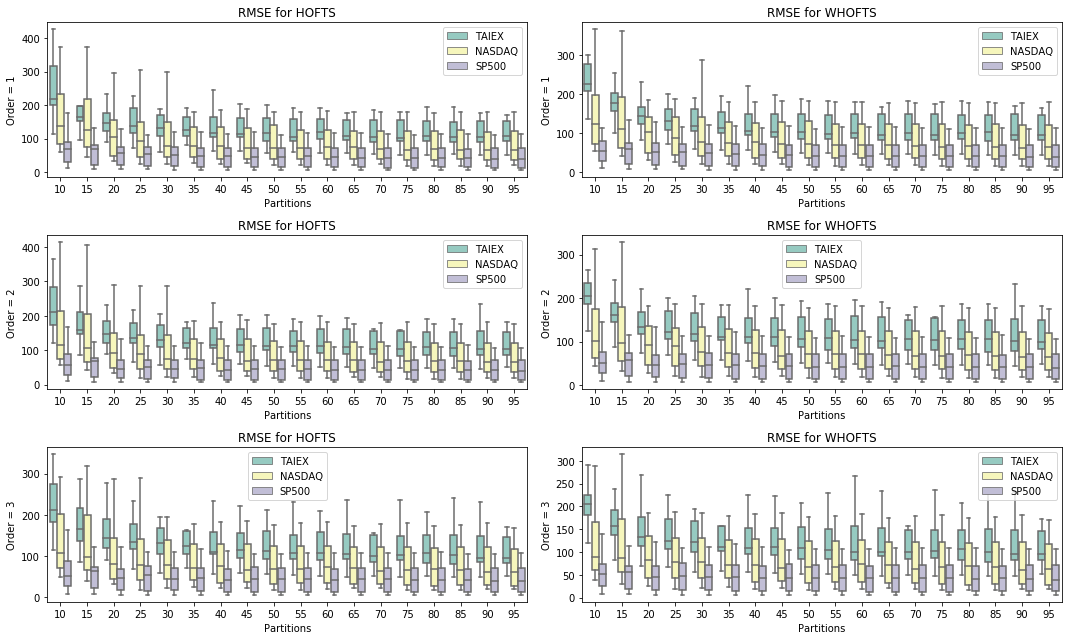
\includegraphics[width=\textwidth, height=12cm]{figures/hofts_gridsearch.png}
    \caption{HOFTS and WHOFTS grid search over hyperparameters $k$ and $\Omega$}
    \label{fig:hofts_gridsearch}
\end{figure}


\begin{figure}[htb]
    \centering
    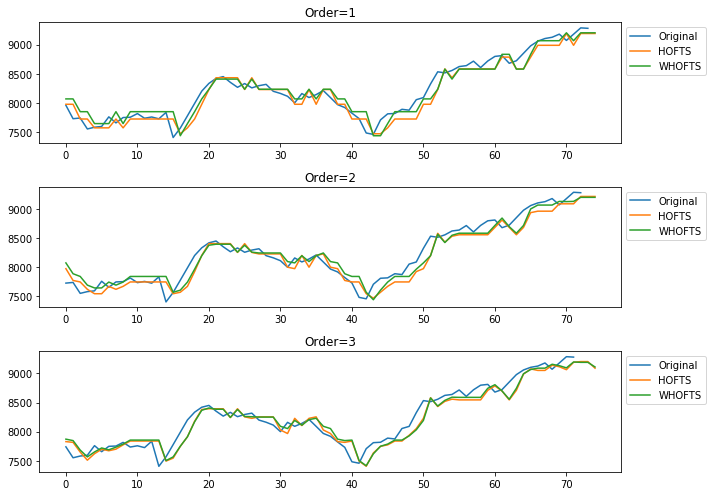
\includegraphics[width=\textwidth]{figures/fts_order.png}
    \caption{The impact of order in forecasting}
    \label{fig:fts_order}
\end{figure}

\begin{figure}[htb]
    \centering
    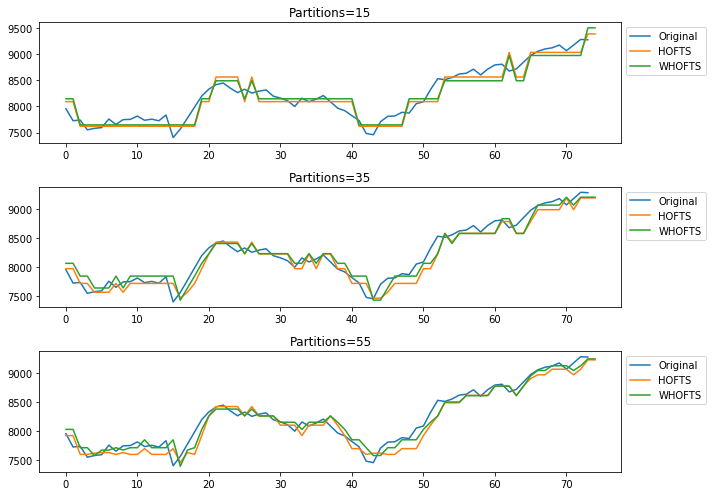
\includegraphics[width=\textwidth]{figures/fts_partitions.png}
    \caption{The impact of partitioning in forecasting}
    \label{fig:fts_partitions}
\end{figure}

%%%%%%%%%%%%%%%%%%%%%%%%%%%%%%%%%%%%%%%%%%%%%%%%%%%%%%%%%%%%%%%%%%%%%%%%%%%%
%%%%%%%%%%%%%%%%%%%%%%%%%%%%%%%%%%%%%%%%%%%%%%%%%%%%%%%%%%%%%%%%%%%%%%%%%%%%
\subsection{Residual Analysis}\index{Residual Analysis}
\label{sec:fts_residual}

The residuals of the models are presented in Figures \ref{fig:hofts_residual} and \ref{fig:whofts_residual} and the Ljung-Box tests for the 3 first lags are presented in Tables \ref{tab:hofts_residuals} and \ref{tab:whofts_residuals}, which show the good fit of model. However, high correlated residuals were detected in some non-stationary sub samples of the datasets, what was also expected since the models are time-invariant. Best performance is expected for time-variant models, capable to adjust its behavior due to changes in data.

\begin{figure}[htb]
    \centering
    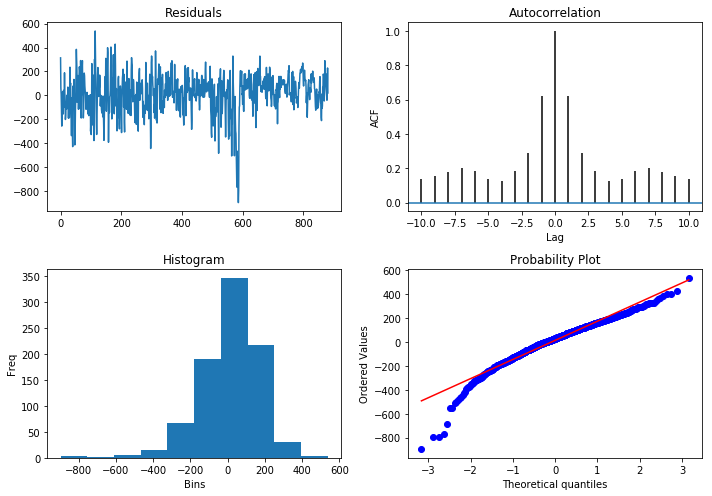
\includegraphics[width=\textwidth,height=7cm]{figures/hofts_residual.png}
    \caption{HOFTS residuals}
    \label{fig:hofts_residual}
\end{figure}

\begin{table}[htb]
    \centering
    \begin{tabular}{|c|c|c|c|c|}
\hline
Lag &   Statistic &  p-Value &  Critical Value &       Result \\ \hline
1 &  341.295085 &      0.0 &        3.841459 &  H0 accepted \\ \hline
2 &  412.500903 &      0.0 &        5.991465 &  H0 accepted \\ \hline
3 &  441.435962 &      0.0 &        7.814728 &  H0 accepted \\ \hline
\end{tabular}
    \caption{Ljung-Box Test for HOFTS residuals}
    \label{tab:hofts_residuals}
\end{table}

\begin{figure}[htb]
    \centering
    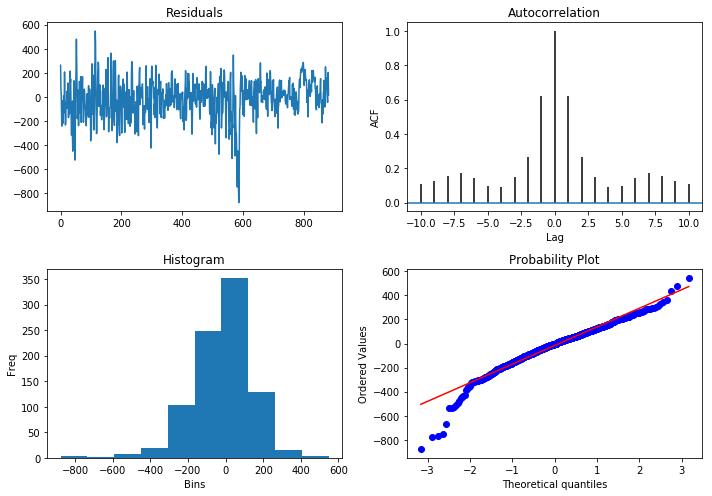
\includegraphics[width=\textwidth,height=7cm]{figures/whofts_residual.png}
    \caption{WHOFTS residuals}
    \label{fig:whofts_residual}
\end{figure}

\begin{table}[htb]
    \centering
    \begin{tabular}{|c|c|c|c|c|}
\hline
Lag &   Statistic &  p-Value &  Critical Value &       Result \\ \hline
1 &  336.838522 &      0.0 &        3.841459 &  H0 accepted \\ \hline
2 &  394.472179 &      0.0 &        5.991465 &  H0 accepted \\ \hline
3 &  411.754344 &      0.0 &        7.814728 &  H0 accepted \\ \hline
\end{tabular}
    \caption{Ljung-Box Test for WHOFTS residuals}
    \label{tab:whofts_residuals}
\end{table}

%%%%%%%%%%%%%%%%%%%%%%%%%%%%%%%%%%%%%%%%%%%%%%%%%%%%%%%%%%%%%%%%%%%%%%%%%%%%
%%%%%%%%%%%%%%%%%%%%%%%%%%%%%%%%%%%%%%%%%%%%%%%%%%%%%%%%%%%%%%%%%%%%%%%%%%%%
\section{Conclusion} 

This chapter provided a brief overview related to the Fuzzy Time Series models. A literature review and some state-of-the-art works related to FTS were presented and summarized in Table \ref{tab:fts_methods}.

The presented methods have some common drawbacks. The matrix-based methods have scalability issues, suffering from the curse of dimensionality. With the rule-based methods, in the forecasting step, just one rule is chosen for computing the result, based on the maximum membership between the input value and all the rules. This causes the loss of ``smoothing'' effect of fuzzy methods, which demands mixing many sets according to their fuzzy membership values. Lastly, these models are point-based forecasters and give no uncertainty measures about their results.  Otherwise, black-box knowledge models eliminate the readability and auditability of the model, and in some cases are not parsimonious. 

To enforce the focus of this research on rule-based FTS methods,  the High Order FTS (HOFTS) and the Weighted High Order FTS (WHOFTS) methods were developed, following a consensus construction from the several approaches present in literature. Computational experiments were employed to assess the point forecasting performance of the methods using financial datasets.

It is necessary to highlight the absence of probabilistic forecasting methods in the Fuzzy Time Series literature. These methods will be discussed in next chapter, where their main features are pointed out and a new method for interval-forecasting with FTS is proposed. 

\begin{center}
    \begin{landscape}
\begin{longtable}[c]{|m{4cm}|c|c|c|c|c|c|c|c|c|m{5cm}|} \hline
\textbf{Reference}   & $n$ & $\Pi$ & $\mu$ & \textbf{Fuzz.} & $\Omega$ & \textbf{Ind.} & \textbf{$\model$}      & \textbf{Transf.} & \textbf{Defuzz.} & \textbf{Application}  \\ \hline \hline
\endhead
%
\cite{song1993fuzzy}      & 1                  & G                  & Tri  & Max                & 1              & H                       & M              & -                        & SM              & Enrollments           \\ \hline
\cite{chen1996forecasting} & 1                  & G                  & Tri  & Max                & 1              & H                       & R               & -                        & SM              & Enrollments           \\ \hline
\cite{Chang1997}           & 1                  & H             & Tri  & All                    & S       & O                    & P          & -                        & -                        & Sales                 \\ \hline
\cite{Song1997}            & 1                  & G                  & Tri  & Max                & 1              & H                       & M              & -                        & -                        & -                     \\ \hline
\cite{Tseng1999}           & 1                  & G                  & Tri  & Max                & S       & O                   & P           & -                        & -                        & Industrial Production \\ \hline
\cite{Song1999}            & 1                  & G                  & Tri  & Max                & S       & H                       & M              & -                        & SM              & -                     \\ \hline
\cite{Chen2000}            & 2                  & G                  & Tri  & Max                & 1              & H                       & M              & -                        & WS            & Temperature           \\ \hline
\cite{huarng2001effective} & 1                  & H             & Tri  & Max                & 1              & H                       & R               & -                        & SM              & Stock Price           \\ \hline
\cite{Chen2002}            & 1                  & G                  & Tri  & Max                & 5              & H                       & R              & -                        & SM              & Enrollments           \\ \hline
\cite{Huarng2004}          & 1                  & H             & Tri  & Max                & 1              & H                       & R               & -                        & SM              & Stock Price           \\ \hline
\cite{yu2005weighted}              & 1                  & G                  & Tri  & Max                & 1              & H                       & WR      & -                        & WS            & Stock Price           \\ \hline
\cite{Huarng2006}          & 1                  & G                  & Tri  & Max                & 1              & BP                              & NN                 & -                        & SM              & Stock Price           \\ \hline
\cite{Chen2006a}           & 1                  & MH         & Tri  & Max                & 3              & H                       & M              & -                        & SM              & Enrollments           \\ \hline
\cite{Lee2006}             & 4                  & G                  & -           & Max                & 1              & H                       & R               & -                        & SM              & Stock Price           \\ \hline
\cite{Cheng2006a}          & 1                  & E               & Trap & Max                & 1              & H                       & M              & -                        & SM              & Project Cost          \\ \hline
\cite{Cheng2008}          & 1                  & E               & Trap & Max                & 1              & H                       & M              & -                        & WS            & Outpatient visits     \\ \hline
\cite{Cheng2008a}           & 1                  & G                  & -           & -                      & 1              & H                       & WR      & D, AE           & WS            & Stock Price           \\ \hline
\cite{Jilani2008a}         & 6                  & G                  & Tri  & Max                & 4              & H                       & M              & -                        & WS            & -                     \\ \hline
\cite{Li2008b}             & 2                  & C            & FCM         & All                    & 2              & H                       & R                & -                        & SM              & Temperature           \\ \hline
\cite{Davari2009}          & 2                  & MH         & Tri  & Max                & 1              & H                       & M              & -                        & WS            & Enrollments           \\ \hline
\cite{Kuo2009}             & 1                  & MH         & -           & -                      & ?              & MH                             & WR      & -                        & ?                        & Enrollments           \\ \hline
\cite{Egrioglu2009}        & 2                  & G                  & Trap & All                    & 3              & BP                              & NN                 & -                        & SM              & Accident              \\ \hline
\cite{Hsu2010}             & 2                  & MH         & -           & Max                & 1              & H                       & R               & -                        & SM              & Temperature           \\ \hline
\cite{Chen2011}            & 2                  & -                     & -           & -                      & ?              & H                       & WR      & D                     & -                        & Stock Price           \\ \hline
\cite{Huang2011}           & 1                  & MH   & Tri  & Max                & 3              & H                       & R               & AE                 & WS            & Enrollments           \\ \hline
\cite{Lee2011}             & 1                  & G                  & -           & -                      & S       & H                       & WR      & D                     & -                        & Stock Price           \\ \hline
\cite{ismail2011enrollment}          & 1                  & G                  & -           & Max                & 1              & H                       & WR      & -                        & WS            & Enrollments           \\ \hline
\cite{Cheng2012}           & 1                  & -                     & -           & -                      & ?              & H                       & WR      & ?                        & -                        & -                     \\ \hline
\cite{Enayatifar2013}      & 1                  & MH         & -           & -                      & 3              & MH                   & WR      & AE                 & -                        & Energy Load           \\ \hline
\cite{Lee2013}             & 1                  & G                  & -           & -                      & 1              & H                       & WR      & BC                  & WS            & Stock Price           \\ \hline
\cite{Chen2014}            & 1                  & E               & -           & -                      & 2              & H                       & WR      & ?                        & -                        & Stock Price           \\ \hline
\cite{Sadaei2014a}          & 1                  & -                     & -           & Max                & 1              & H                       & WR      & ROI, AE            & WS            & Stock Price           \\ \hline
\cite{Askari2015}          & 3                  & C            & FCM         & All                    & 1              & H                       & P & -                        & WS            & Stock Price           \\ \hline
\cite{Bas2015}             & 1                  & C            & FCM         & All                    & 1              & MH                             & NN                 & -                        & WS            & Stock Price           \\ \hline
\cite{Cai2015}             & 1                  & MHs        & trmf        & All                    & 1              & H                       & WR      & -                        & WS            & Stock Price           \\ \hline
\cite{Chen2015a}           & 2                  & G                  & Tri  & Max                & 2              & H                       & R               & -                        & WS            & Stock Price           \\ \hline
\cite{Ismail2015}          & 1                  & Q              & -           & -                      & 1              & H                       & M              & -                        & SM              & Energy Load           \\ \hline
\cite{Sun2015}             & 3                  & C            & FCM         & All                    & 1              & H                       & R                & -                        & WS            & Stock Price           \\ \hline
\cite{Singh2015}           & 3                  & G                  & -           & Max                & 1              & BP                             & NN                 & AE             & WS            & Stock price           \\ \hline
\cite{Rubio2016}           & 1                  & H             & Trap & All                    & 1              & H                       & M              & -                        & WS            & Portfolio returns     \\ \hline
\cite{Sadaei2016}          & 1                  & G                  & Tri  & Max                & 1              & H                       & R               & D, AE           & SM              & Stock Price           \\ \hline
\cite{Talarposhti2016a}    & 1                  & MH         & Tri  & Max                & 1              & H                       & P  & -                        & WS            & Stock Price           \\ \hline
\cite{Ye2016}              & 1                  & G                  & Tri  & AC              & 3              & MH                         & M              & ROC, AE            & WS            & Sock price            \\ \hline
\cite{Lee2017}             & 1                  & G                  & Tri  & Max                & 3              & H                     & R               & -                        & WS            & Enrollments           \\ \hline
\cite{Yang2017}            & 3                  & CS            & Tri  & Max                & 1              & H                       & R               & EMD, AE            & SM              & Wind Speed            \\ \hline
\cite{Yolcu2017}           & 1                  & C            & FCM         & All                    & 1              & MH                             & MLP                 & -                        & WS            & Sock price            \\ \hline
\cite{Bose2017}            & 1                  & C            & Tri  & -                      & 3              & H                       & R                & AE                 & WS            & -                     \\ \hline
\cite{CarvalhoJr2017}      & 1                  & G                  & Tri  & AC              & 1              & H                       & R               & -                        & SM              & Stock price           \\ \hline
\cite{Jiang2017}           & 1                  & MH         & Tri  & Max                & 3              & H                       & WR      & -                        & WS            & Stock price           \\ \hline
\cite{Saberi2017}          & 1                  & C            & fefts       & All                    & 1              & H                       & M              & -                        & WS            & -                     \\ \hline
\cite{Sadaei2017}          & 1                  & MH         & Tri  & Max                & *              & O                         & P      & -                        & ?                        & Energy Load           \\ \hline
\cite{Severiano2017a}      & 1                  & G                  & Tri  & All                    & 3              & H                       & R               & -                        & SM              & Energy Load           \\ \hline
\cite{Bas2018}             & 1                  & C            & FCM         & All                    & 1              & P                             & NN               & -                        & WS            & Stock price           \\ \hline
\cite{Guney2018}           & 1                  & G                  & Tri  & Max                & 2              & H                       & MC        & -                        & WS            & -                     \\ \hline
\cite{Cheng2018}           & 1                  & H             & Trap & Max                & 3              & A                         & R                & -                        & WS            & Stock price           \\ \hline
\cite{Dincer2018}          & 1                  & C            & -           & Max                & 1              & H                       & M              & -                        & SM              & Air pollution         \\ \hline
\cite{Yang2018}            & 5                  & MH         & Trap & Max                &                & MH                   & P  & EMD                      & WS            & Stock price           \\ \hline
\cite{Yang2018}            & 5                  & C            & -           & -                      & 2              & RG                      & FCM                 & WV                 & WS            & -                     \\ \hline
\cite{Tran2018}            & 3                  & C            & -           & All                    & 1              & BP                            & NN                & N            & WS            & -                     \\ \hline
\cite{Zhang2018}           & 4                  & H                & FCM         & -                      & 1              & BP                             & NN                 & -                        & WS            & Stock price           \\ \hline
\cite{Zhang2018a}          & 2                  & MH         & Tri  & Max                & 2              & H                       & R               & -                        & SM              & Stock price           \\ \hline
\cite{Chen2019a}            & 1                  & G                  & Trap & Max                & 1              & H                       & M              & -                        & WS            & Flood \\  \hline
\cite{Sadaei2019}            & 1                  & G                  & Tri & Max                &  *              & BP                       & NN              & -                        & WS            & Energy Load \\  \hline
\multicolumn{11}{l}{$\mathbf{n}$\textbf{ - Number of variables}} \\
\multicolumn{11}{p{20cm}}{$\mathbf{\Pi}$\textbf{ - Partitioning method}: G - Grid, H - Heuristic, MH - Metaheuristic, CS - Chi-Square, E - Entropy, Q - Quartile} \\
\multicolumn{11}{p{20cm}}{$\mathbf{\mu}$\textbf{ - Membership function}: Tri - Triangular, Trap - Trapezoidal, FCM - Fuzzy C-Means} \\
\multicolumn{11}{p{20cm}}{\textbf{Fuzz - Fuzzyfication method}: Max - Maximum membership, All - All memberships, AC - alpha-cut} \\
\multicolumn{11}{l}{$\mathbf{\Omega}$\textbf{  - Order}} \\
\multicolumn{11}{p{20cm}}{\textbf{Ind. - Knowledge induction method}: H - Heuristic, MH - Metaheuristic, BP - Backpropagation, O - Optimization, RG - Regression analysis, AP - Apriori} \\
\multicolumn{11}{p{20cm}}{$\mathbf{\model}$\textbf{ - Knowledge model}: M - Matrix, R - Rules, WR - Weighted Rules, NN - Neural Network, FCM - Fuzzy Cognitive Map, P - Polynomial, MC - Markov Chain} \\
\multicolumn{11}{p{20cm}}{\textbf{Transf - Transformations}: A - Adaptive expectation; B - Box-Cox;  D - Differentiation; R - ROI, N - Normalization} \\ \hline
\caption{Summary of the most relevant FTS methods}
\label{tab:fts_methods}\\
\end{longtable}
\end{landscape}
\end{center}
